%==============================================================================
% OBJEKTERKENNUNG MIT YOLO
% Durchgehendes Praxisbeispiel: KI-Kasse (Euro-Münzen erkennen und summieren)
%==============================================================================

% ---------------------------------------------------------
% Hilfsmakros für die Münz-Grafiken
% \yoloMuenze{(x,y)}{Radius}{Farbe außen}{Farbe innen}{Beschriftung}
% \yoloBox{(x,y)}{halbe Kantenlänge}{Farbe}{Label}
% ---------------------------------------------------------
\colorlet{KupferColor}{AlertColor!55!AccentColor!45}
\colorlet{GoldColor}{AccentColor!55}
\colorlet{SilberColor}{DarkGrey!25}

\newcommand{\yoloMuenze}[5]{%
  \filldraw[fill=#3, draw=#3!60!black, line width=0.6pt] #1 circle (#2);
  \filldraw[fill=#4, draw=#4!60!black, line width=0.3pt] #1 circle ({0.72*#2});
  \node[font=\tiny\bfseries, text=TextColor] at #1 {#5};%
}
\newcommand{\yoloBox}[4]{%
  \draw[#3, line width=1pt] ($#1+(-#2-0.06,-#2-0.06)$) rectangle ($#1+(#2+0.06,#2+0.06)$);
  \node[fill=#3, text=white, font=\tiny\bfseries, inner sep=1pt, anchor=south west]
    at ($#1+(-#2-0.06,#2+0.06)$) {#4};%
}
% Beispielszene: fünf Münzen auf einem Tisch (6 x 4,5 Einheiten)
\newcommand{\yoloSzene}{%
  \fill[DarkGrey!8] (0,0) rectangle (6,4.5);
  \draw[DarkGrey!60] (0,0) rectangle (6,4.5);
  \yoloMuenze{(1.4,3.0)}{0.65}{SilberColor}{GoldColor}{2\,€}
  \yoloMuenze{(3.3,1.4)}{0.62}{GoldColor}{GoldColor}{50\,ct}
  \yoloMuenze{(4.7,3.2)}{0.50}{GoldColor}{GoldColor}{10\,ct}
  \yoloMuenze{(1.5,1.0)}{0.42}{KupferColor}{KupferColor}{1\,ct}
  \yoloMuenze{(4.9,1.2)}{0.58}{GoldColor}{SilberColor}{1\,€}%
}

\makesectionpage{Objekterkennung mit YOLO}

\makesubsectionpage{Von der Klassifikation zur Objekterkennung}

% ---------------------------------------------------------
\begin{frame}{Objekterkennung: Motivation}
\begin{columns}
\begin{column}{0.60\textwidth}
\begin{itemize}
  \item Bisher: \textbf{Bildklassifikation}, ein Bild erhält genau \textbf{ein Label}.
  \item VGG16 erkennt eine Katze auf einem Bild, sagt aber nicht, \textbf{wo} sie ist.
  \item Reale Bilder enthalten \textbf{mehrere Objekte} unterschiedlicher Klassen.
  \item \textbf{Objekterkennung} beantwortet drei Fragen gleichzeitig:
  \begin{itemize}
    \item Welche Objekte sind zu sehen?
    \item Wo liegen sie?
    \item Wie viele sind es?
  \end{itemize}
  \item Anwendungen: autonomes Fahren, Qualitätskontrolle, Medizin, Einzelhandel
\end{itemize}
\end{column}
\begin{column}{0.35\textwidth}
\centering
\resizebox{0.9\linewidth}{!}{%
\begin{tikzpicture}
  \yoloSzene
  \yoloBox{(1.4,3.0)}{0.65}{PrimaryColor}{2\,€ 0,94}
  \yoloBox{(3.3,1.4)}{0.62}{ThirdColor}{50\,ct 0,88}
  \yoloBox{(4.7,3.2)}{0.50}{ExampleColor}{10\,ct 0,81}
  \yoloBox{(1.5,1.0)}{0.42}{AlertColor}{1\,ct 0,67}
  \yoloBox{(4.9,1.2)}{0.58}{AccentColor!80!black}{1\,€ 0,91}
  \node[font=\small\bfseries, anchor=north] at (3,-0.15) {Summe: 3,61\,€};
\end{tikzpicture}%
}
\end{column}
\end{columns}
\end{frame}

% ---------------------------------------------------------
\begin{frame}{Aufgaben der Bildanalyse}
\begin{columns}
\begin{column}{0.35\textwidth}
\begin{itemize}
  \item \textbf{Klassifikation:} Was ist auf dem Bild?
  \item \textbf{Lokalisierung:} Wo liegt das eine Objekt?
  \item \textbf{Objekterkennung:} Alle Objekte mit Klasse und Bounding Box
  \item \textbf{Instanzsegmentierung:} Pixelgenaue Maske je Objekt
\end{itemize}
\vfill
YOLO beherrscht alle vier Aufgaben. Im Fokus steht hier die \textbf{Objekterkennung}.
\end{column}
\begin{column}{0.60\textwidth}
\centering
\resizebox{0.9\linewidth}{!}{%
\begin{tikzpicture}
  % Klassifikation
  \begin{scope}[shift={(0,5.6)}]
    \fill[DarkGrey!8] (0,0) rectangle (6,4.5);
    \draw[DarkGrey!60] (0,0) rectangle (6,4.5);
    \yoloMuenze{(3,2.25)}{1.3}{SilberColor}{GoldColor}{}
    \node[font=\bfseries] at (3,2.25) {2\,€};
    \node[anchor=north] at (3,-0.1) {\textbf{Klassifikation:} „2\,€“};
  \end{scope}
  % Lokalisierung
  \begin{scope}[shift={(6.8,5.6)}]
    \fill[DarkGrey!8] (0,0) rectangle (6,4.5);
    \draw[DarkGrey!60] (0,0) rectangle (6,4.5);
    \yoloMuenze{(3.6,2.0)}{1.0}{SilberColor}{GoldColor}{}
    \node[font=\bfseries] at (3.6,2.0) {2\,€};
    \yoloBox{(3.6,2.0)}{1.0}{PrimaryColor}{2\,€}
    \node[anchor=north] at (3,-0.1) {\textbf{Lokalisierung}};
  \end{scope}
  % Objekterkennung
  \begin{scope}[shift={(0,0)}]
    \yoloSzene
    \yoloBox{(1.4,3.0)}{0.65}{PrimaryColor}{2\,€}
    \yoloBox{(3.3,1.4)}{0.62}{ThirdColor}{50\,ct}
    \yoloBox{(4.7,3.2)}{0.50}{ExampleColor}{10\,ct}
    \yoloBox{(1.5,1.0)}{0.42}{AlertColor}{1\,ct}
    \yoloBox{(4.9,1.2)}{0.58}{AccentColor!80!black}{1\,€}
    \node[anchor=north] at (3,-0.1) {\textbf{Objekterkennung}};
  \end{scope}
  % Instanzsegmentierung
  \begin{scope}[shift={(6.8,0)}]
    \yoloSzene
    \fill[PrimaryColor, opacity=0.45] (1.4,3.0) circle (0.65);
    \fill[ThirdColor, opacity=0.45] (3.3,1.4) circle (0.62);
    \fill[ExampleColor, opacity=0.45] (4.7,3.2) circle (0.50);
    \fill[AlertColor, opacity=0.45] (1.5,1.0) circle (0.42);
    \fill[AccentColor, opacity=0.55] (4.9,1.2) circle (0.58);
    \node[anchor=north] at (3,-0.1) {\textbf{Instanzsegmentierung}};
  \end{scope}
\end{tikzpicture}%
}
\end{column}
\end{columns}
\end{frame}

% ---------------------------------------------------------
\begin{frame}{Unser Projekt: Die KI-Kasse}
\footnotesize
\setbeamerfont{block title}{size=\footnotesize}
\begin{columns}
\begin{column}{0.47\textwidth}
\begin{itemize}
  \item \textbf{Ziel:} Münzen liegen unter einer Kamera, das System zeigt \textbf{live die Summe} an.
  \item Kamera $\rightarrow$ YOLO $\rightarrow$ Detektionen $\rightarrow$ Summe
  \item \textbf{8 Klassen:} 1, 2, 5, 10, 20 und 50 Cent sowie 1\,€ und 2\,€
  \item Das Ergebnis ist im Hörsaal \textbf{sofort überprüfbar}.
  \item Herausforderungen:
  \footnotesize
  \begin{itemize}
    \item Sehr ähnliche Klassen
    \item Unterschiedliche nationale Rückseiten
    \item Spiegelungen, Abnutzung, Überlappungen
    \item Größe hilft nur bei \textbf{fester Kamerahöhe}
  \end{itemize}
\end{itemize}
\end{column}
\begin{column}{0.48\textwidth}
\centering
\begin{tabular}{lrl}
\toprule
\textbf{Münze} & \textbf{Ø in mm} & \textbf{Farbe} \\
\midrule
1\,ct  & 16,25 & Kupfer \\
2\,ct  & 18,75 & Kupfer \\
10\,ct & 19,75 & Gold \\
5\,ct  & 21,25 & Kupfer \\
20\,ct & 22,25 & Gold \\
1\,€   & 23,25 & Gold/Silber \\
50\,ct & 24,25 & Gold \\
2\,€   & 25,75 & Silber/Gold \\
\bottomrule
\end{tabular}

\vspace{0.6em}
Nach Größe sortiert wechseln sich die Farben ab. Das Netz muss \textbf{Größe, Farbe und Prägung} kombinieren.
\end{column}
\end{columns}
\source{\cite{bundesbank_euromuenzen}}
\end{frame}

% ---------------------------------------------------------
\begin{frame}{Naiver Ansatz: Sliding Window}
\footnotesize
\begin{columns}
\begin{column}{0.60\textwidth}
\begin{itemize}
  \item Ein \textbf{Fenster} gleitet über das Bild, jeder Ausschnitt wird mit einem CNN \textbf{klassifiziert}.
  \item \textbf{Mehrere Fenstergrößen} sind nötig, z.\,B. bei $640 \times 640$ Pixeln und Stride $16$:
\end{itemize}
\begin{center}
\begin{tabular}{lrrrr}
\toprule
\textbf{Fenster} & $64^2$ & $128^2$ & $256^2$ & \textbf{Summe} \\
\midrule
\textbf{Ausschnitte} & \num{1369} & \num{1089} & 625 & \textbf{\num{3083}} \\
\bottomrule
\end{tabular}
\end{center}
\begin{itemize}
  \item VGG16: ca. 15,5 Mrd. Multiply-Add-Operationen je Ausschnitt, also rund \textbf{48 Billionen pro Bild}
  \item YOLO26n: 5,5 Mrd. FLOPs für das \textbf{ganze Bild}, Faktor \textbf{über \num{10000}}
  \item Zusätzlich: feste Seitenverhältnisse, ungenaue Boxen, Doppeltreffer
\end{itemize}
\end{column}
\begin{column}{0.35\textwidth}
\centering
\resizebox{0.9\linewidth}{!}{%
\begin{tikzpicture}
  \yoloSzene
  \draw[AlertColor, line width=1pt, dashed] (0.2,2.4) rectangle (1.4,3.6);
  \draw[AlertColor!60, line width=0.6pt, dashed] (0.6,2.4) rectangle (1.8,3.6);
  \draw[AlertColor!35, line width=0.6pt, dashed] (1.0,2.4) rectangle (2.2,3.6);
  \draw[PrimaryColor, line width=1pt, dashed] (2.4,0.4) rectangle (4.4,2.4);
  \draw[ExampleColor, line width=1pt, dashed] (3.9,2.6) rectangle (5.5,3.9);
  \draw[-{Latex[length=2mm]}, AlertColor, line width=0.8pt] (0.3,3.8) -- (2.0,3.8);
  \node[font=\scriptsize, anchor=north] at (3,-0.1) {Fenster in drei Größen};
\end{tikzpicture}%
}

\vspace{1em}
\raggedright
\textbf{YOLO, You Only Look Once:} Ein einziger Durchlauf durch das Netz liefert alle Boxen und Klassen.
\end{column}
\end{columns}
\source{\cite{simonyan2014vgg, redmon2016yolo, ultralytics_yolo26}}
\end{frame}

\makesubsectionpage{Grundbegriffe der Objekterkennung}

% ---------------------------------------------------------
\begin{frame}{Bounding Boxes: Darstellungsformen}
\footnotesize
\begin{columns}
\begin{column}{0.47\textwidth}
\begin{itemize}
  \item Bildkoordinaten: Ursprung \textbf{oben links}, $y$ wächst nach \textbf{unten}.
  \item Drei gängige Formate:
\end{itemize}
\begin{center}
\begin{tabular}{ll}
\toprule
\textbf{Format} & \textbf{Werte} \\
\midrule
xyxy (Pascal VOC) & $(x_1, y_1, x_2, y_2)$ \\
xywh (COCO) & $(x_1, y_1, w, h)$ \\
YOLO & $(x_c, y_c, w, h) \in [0,1]^4$ \\
\bottomrule
\end{tabular}
\end{center}
\begin{itemize}
  \item YOLO-Labels sind auf Bildbreite und Bildhöhe \textbf{normiert} und damit unabhängig von der Auflösung.
  \item Ultralytics liefert beide Varianten: \texttt{boxes.xyxy} in Pixeln, \texttt{boxes.xywhn} normiert
\end{itemize}
\end{column}
\begin{column}{0.48\textwidth}
\centering
\resizebox{0.9\linewidth}{!}{%
\begin{tikzpicture}[yscale=-1]
  \fill[DarkGrey!8] (0,0) rectangle (6,4.5);
  \draw[DarkGrey!60] (0,0) rectangle (6,4.5);
  \draw[-{Latex[length=2mm]}, line width=0.8pt] (0,0) -- (6.5,0) node[right] {$x$};
  \draw[-{Latex[length=2mm]}, line width=0.8pt] (0,0) -- (0,5.0) node[below] {$y$};
  \node[above left] at (0,0) {$(0,0)$};
  \node[below right, font=\footnotesize] at (6,4.5) {$(W,H)$};
  \yoloMuenze{(3.6,2.5)}{1.0}{SilberColor}{GoldColor}{2\,€}
  \draw[PrimaryColor, line width=1.2pt] (2.5,1.4) rectangle (4.7,3.6);
  \fill[PrimaryColor] (2.5,1.4) circle (2pt) node[above left] {$(x_1, y_1)$};
  \fill[PrimaryColor] (4.7,3.6) circle (2pt) node[below right] {$(x_2, y_2)$};
  \fill[AlertColor] (3.6,2.5) circle (2pt);
  \node[AlertColor, font=\footnotesize, anchor=west] at (3.65,2.75) {$(x_c, y_c)$};
  \draw[{Latex[length=1.5mm]}-{Latex[length=1.5mm]}, ExampleColor!80!black] (2.5,3.85) -- node[below] {$w$} (4.7,3.85);
  \draw[{Latex[length=1.5mm]}-{Latex[length=1.5mm]}, ExampleColor!80!black] (2.25,1.4) -- node[left] {$h$} (2.25,3.6);
\end{tikzpicture}%
}

\footnotesize
\textbf{Hinweis: } $x_c, y_c$  sind bei YOLO der Mittelpunkt der Bounding Box.

\end{column}
\end{columns}
\end{frame}

% ---------------------------------------------------------
\begin{frame}{Umrechnung ins YOLO-Format}
\footnotesize
\setbeamerfont{block title}{size=\footnotesize}
\begin{columns}
\begin{column}{0.47\textwidth}
Von xyxy in Pixeln zu YOLO, Bildgröße $W \times H$:
\begin{align*}
x_c &= \frac{x_1 + x_2}{2W}, & y_c &= \frac{y_1 + y_2}{2H}, \\[2pt]
w   &= \frac{x_2 - x_1}{W},  & h   &= \frac{y_2 - y_1}{H}.
\end{align*}
Rückrichtung:
\begin{align*}
x_1 &= \left(x_c - \tfrac{w}{2}\right) W, & y_1 &= \left(y_c - \tfrac{h}{2}\right) H, \\[2pt]
x_2 &= \left(x_c + \tfrac{w}{2}\right) W, & y_2 &= \left(y_c + \tfrac{h}{2}\right) H.
\end{align*}
\begin{itemize}
  \item Pro Bild eine Textdatei, pro Objekt eine Zeile
  \item Klassen-IDs beginnen bei $0$.
\end{itemize}
\end{column}
\begin{column}{0.48\textwidth}
\begin{beispiel}[2-€-Münze im YOLO-Format\strut]
Bild mit $1280 \times 960$ Pixeln, Box $(512, 384, 640, 512)$, Klasse 2\,€ hat die ID $7$:
\begin{align*}
x_c &= \tfrac{512 + 640}{2 \cdot 1280} = 0{,}450, & y_c &= \tfrac{384 + 512}{2 \cdot 960} \approx 0{,}467, \\[2pt]
w   &= \tfrac{640 - 512}{1280} = 0{,}100, & h &= \tfrac{512 - 384}{960} \approx 0{,}133.
\end{align*}
Zeile in der Labeldatei:

\centering
\texttt{7 0.450 0.467 0.100 0.133}
\end{beispiel}
\end{column}
\end{columns}
\source{\cite{ultralytics_datasets_detect}}
\end{frame}

% ---------------------------------------------------------
\begin{frame}{Intersection over Union (IoU)}
\footnotesize
\setbeamerfont{block title}{size=\footnotesize}
\begin{columns}
\begin{column}{0.60\textwidth}
\begin{definition}[Intersection over Union\strut]
Für zwei Boxen $A$ und $B$ ist
\[
\operatorname{IoU}(A, B) = \frac{|A \cap B|}{|A \cup B|} = \frac{|A \cap B|}{|A| + |B| - |A \cap B|}.
\]
\end{definition}
\begin{itemize}
  \item Wertebereich $[0, 1]$: $0$ bei keiner Überlappung, $1$ bei identischen Boxen
  \item Misst, wie gut eine \textbf{Vorhersage} zur \textbf{Ground Truth} passt
  \item Übliche Schwelle: $\operatorname{IoU} \geq 0{,}5$ gilt als Treffer.
  \item Grundlage für \textbf{NMS} und die Metrik \textbf{mAP}
\end{itemize}
\end{column}
\begin{column}{0.35\textwidth}
\centering
\resizebox{0.9\linewidth}{!}{%
\begin{tikzpicture}
  % Boxen
  \fill[AccentColor!45] (1.2,0.8) rectangle (3,2.5);
  \draw[ExampleColor, line width=1.4pt] (0,0) rectangle (3,2.5);
  \draw[AlertColor, line width=1.4pt, dashed] (1.2,0.8) rectangle (4.2,3.3);
  \node[ExampleColor!80!black, font=\small\bfseries, anchor=north west] at (0,0) {Ground Truth};
  \node[AlertColor, font=\small\bfseries, anchor=south east] at (4.2,3.3) {Vorhersage};
  \node[font=\small\bfseries] at (2.1,1.65) {$A \cap B$};
\end{tikzpicture}%
}
\end{column}
\end{columns}
\end{frame}

% ---------------------------------------------------------
\begin{frame}{IoU: Berechnung für achsenparallele Boxen}
\footnotesize
\setbeamerfont{block title}{size=\footnotesize}
\begin{columns}
\begin{column}{0.47\textwidth}
Boxen im Format xyxy, Schnittrechteck:
\begin{align*}
x_1^{\cap} &= \max(x_1^A, x_1^B), & y_1^{\cap} &= \max(y_1^A, y_1^B), \\
x_2^{\cap} &= \min(x_2^A, x_2^B), & y_2^{\cap} &= \min(y_2^A, y_2^B).
\end{align*}
Schnittfläche:
\[
|A \cap B| = \max(0,\, x_2^{\cap} - x_1^{\cap}) \cdot \max(0,\, y_2^{\cap} - y_1^{\cap})
\]
\begin{itemize}
  \item $\max(0, \cdot)$ fängt den Fall \textbf{ohne Überlappung} ab.
  \item Konstanter Aufwand $O(1)$ pro Boxpaar
\end{itemize}
\end{column}
\begin{column}{0.48\textwidth}
\begin{beispiel}[IoU berechnen\strut]
Ground Truth $A = (100, 100, 200, 200)$, \\
Vorhersage $B = (120, 110, 220, 210)$:
\begin{align*}
A \cap B &= (120, 110, 200, 200), \\
|A \cap B| &= 80 \cdot 90 = \num{7200}, \\
|A| = |B| &= 100 \cdot 100 = \num{10000}, \\
|A \cup B| &= \num{20000} - \num{7200} = \num{12800}, \\
\operatorname{IoU}(A, B) &= \tfrac{\num{7200}}{\num{12800}} \approx 0{,}56.
\end{align*}
\end{beispiel}
\end{column}
\end{columns}
\end{frame}

% ---------------------------------------------------------
\begin{frame}{IoU bei kleinen Objekten}
\footnotesize
\setbeamerfont{block title}{size=\footnotesize}
\begin{columns}
\begin{column}{0.60\textwidth}
Beide Vorhersagen sind um \textbf{4 Pixel} in $x$- und $y$-Richtung verschoben:

\vspace{0.5em}
\begin{blockrow}
  \begin{blockcol}{0.48\linewidth}{blockC1}{2-€-Münze, $100 \times 100$ Pixel}
    \begin{itemize}
      \item Schnitt: $96 \cdot 96 = \num{9216}$
      \item Vereinigung: $\num{20000} - \num{9216} = \num{10784}$
      \item $\operatorname{IoU} \approx \textbf{0{,}85}$
    \end{itemize}
  \end{blockcol}
  \begin{blockcol}{0.48\linewidth}{blockC2}{1-ct-Münze, $20 \times 20$ Pixel}
    \begin{itemize}
      \item Schnitt: $16 \cdot 16 = 256$
      \item Vereinigung: $800 - 256 = 544$
      \item $\operatorname{IoU} \approx \textbf{0{,}47}$
    \end{itemize}
  \end{blockcol}
\end{blockrow}
\end{column}
\begin{column}{0.35\textwidth}
\begin{itemize}
  \item Gleicher Pixelfehler, sehr \textbf{unterschiedliche IoU}
  \item Die 1-ct-Münze gilt bei der Schwelle $0{,}5$ als \textbf{nicht erkannt}.
  \item Kleine Objekte erfordern:
  \footnotesize
  \begin{itemize}
    \item Höhere Eingabeauflösung (\texttt{imgsz})
    \item Kamera näher am Objekt
    \item Besonders sorgfältige Annotation
  \end{itemize}
\end{itemize}
\end{column}
\end{columns}
\end{frame}

% ---------------------------------------------------------
\begin{frame}{Confidence Score}
\footnotesize
\begin{columns}
\begin{column}{0.47\textwidth}
\begin{itemize}
  \item Jede Vorhersage besteht aus \textbf{Box}, \textbf{Klasse} und \textbf{Confidence} $\in [0, 1]$.
  \item YOLOv1: $P(\text{Klasse} \mid \text{Objekt}) \cdot P(\text{Objekt}) \cdot \operatorname{IoU}$
  \item Aktuelle YOLO-Versionen geben direkt einen \textbf{Klassenwert} je Box aus.
  \item Schwellenwert \texttt{conf}: Vorhersagen darunter werden verworfen, Ultralytics-Standard ist $0{,}25$.
  \item \textbf{Zielkonflikt:} Ein hoher Schwellenwert erzeugt weniger Fehlalarme, aber mehr übersehene Münzen.
\end{itemize}
\end{column}
\begin{column}{0.48\textwidth}
\centering
\begin{tabular}{llcc}
\toprule
\textbf{Klasse} & \textbf{Conf.} & $\geq 0{,}25$ & $\geq 0{,}5$ \\
\midrule
2\,€  & 0,94 & $\checkmark$ & $\checkmark$ \\
50\,ct & 0,81 & $\checkmark$ & $\checkmark$ \\
10\,ct & 0,47 & $\checkmark$ & $\times$ \\
1\,ct  & 0,31 & $\checkmark$ & $\times$ \\
20\,ct (Knopf) & 0,28 & $\checkmark$ & $\times$ \\
\midrule
\textbf{Summe} & & 2,81\,€ & 2,50\,€ \\
\bottomrule
\end{tabular}

\vspace{0.8em}
Richtig wären \textbf{2,61\,€}. Keiner der beiden Schwellenwerte liefert das korrekte Ergebnis.
\end{column}
\end{columns}
\source{\cite{redmon2016yolo, ultralytics_cfg}}
\end{frame}

% ---------------------------------------------------------
\begin{frame}{Mehrfachdetektionen}
\begin{columns}
\begin{column}{0.47\textwidth}
\begin{itemize}
  \item Detektoren liefern pro Objekt oft \textbf{viele überlappende Boxen}.
  \item Ursache: Mehrere Stellen der Ausgabe „sehen“ dieselbe Münze.
  \item Für die KI-Kasse fatal: Die 2-€-Münze wird \textbf{dreifach gezählt}.
  \item \textbf{Non-Maximum Suppression (NMS):} Pro Objekt bleibt die Box mit der \textbf{höchsten Confidence}, stark überlappende Boxen derselben Klasse werden entfernt.
\end{itemize}
\end{column}
\begin{column}{0.48\textwidth}
\centering
\resizebox{0.9\linewidth}{!}{%
\begin{tikzpicture}
  % vorher
  \fill[DarkGrey!8] (0,0) rectangle (3.4,3.4);
  \draw[DarkGrey!60] (0,0) rectangle (3.4,3.4);
  \yoloMuenze{(1.7,1.6)}{1.0}{SilberColor}{GoldColor}{2\,€}
  \draw[AlertColor!70, line width=0.9pt] (0.5,0.4) rectangle (2.7,2.6);
  \draw[ThirdColor, line width=0.9pt] (0.8,0.7) rectangle (3.0,2.9);
  \draw[PrimaryColor, line width=1.2pt] (0.62,0.52) rectangle (2.78,2.68);
  \node[font=\tiny, fill=AlertColor!70, text=white, inner sep=1pt, anchor=north west] at (0.5,0.4) {0,62};
  \node[font=\tiny, fill=ThirdColor, text=white, inner sep=1pt, anchor=south east] at (3.0,2.9) {0,84};
  \node[font=\tiny, fill=PrimaryColor, text=white, inner sep=1pt, anchor=south west] at (0.62,2.68) {0,91};
  \node[anchor=north, font=\small] at (1.7,-0.45) {Summe: \textbf{6,00\,€}};
  % Pfeil
  \draw[-{Latex[length=3mm]}, line width=1.5pt] (3.7,1.7) -- node[above, font=\small\bfseries] {NMS} (5.0,1.7);
  % nachher
  \begin{scope}[shift={(5.3,0)}]
    \fill[DarkGrey!8] (0,0) rectangle (3.4,3.4);
    \draw[DarkGrey!60] (0,0) rectangle (3.4,3.4);
    \yoloMuenze{(1.7,1.6)}{1.0}{SilberColor}{GoldColor}{2\,€}
    \draw[PrimaryColor, line width=1.2pt] (0.62,0.52) rectangle (2.78,2.68);
    \node[font=\tiny, fill=PrimaryColor, text=white, inner sep=1pt, anchor=south west] at (0.62,2.68) {0,91};
    \node[anchor=north, font=\small] at (1.7,-0.45) {Summe: \textbf{2,00\,€}};
  \end{scope}
\end{tikzpicture}%
}
\end{column}
\end{columns}
\end{frame}

% ---------------------------------------------------------
\begin{frame}{Non-Maximum Suppression: Algorithmus}
\begin{columns}
\begin{column}{0.35\textwidth}
\begin{itemize}
  \item Greedy-Verfahren, wird \textbf{pro Klasse} ausgeführt
  \item $\tau$: IoU-Schwelle, Ultralytics-Standard bei der Vorhersage ist $0{,}5$
  \item Kleines $\tau$ entfernt mehr Boxen.
  \item Laufzeit $O(n^2)$ für $n$ Boxen
\end{itemize}
\end{column}
\begin{column}{0.60\textwidth}
\begin{algorithm}[H]
\footnotesize
\SetAlCapFnt{\footnotesize}
\SetAlCapNameFnt{\footnotesize}
\KwIn{Boxes $B = \{b_1, \dots, b_n\}$, scores $S$, IoU threshold $\tau$}
\KwOut{Selected boxes $D$}
$D \gets \emptyset$\;
\While{$B \neq \emptyset$}{
  $b^{*} \gets \arg\max_{b \in B} S(b)$\;
  $D \gets D \cup \{b^{*}\}$\;
  $B \gets B \setminus \{b^{*}\}$\;
  \ForEach{$b \in B$}{
    \If{$\operatorname{IoU}(b^{*}, b) \geq \tau$}{
      $B \gets B \setminus \{b\}$\;
    }
  }
}
\Return{$D$}\;
\caption{Non-Maximum Suppression}
\end{algorithm}
\end{column}
\end{columns}
\source{\cite{ultralytics_cfg}}
\end{frame}

% ---------------------------------------------------------
\begin{frame}[fragile]{Implementierung: IoU in Python}
\begin{columns}
\begin{column}{0.60\textwidth}
{\footnotesize
\begin{minted}{python}
def area(r):
    return (r[2] - r[0]) * (r[3] - r[1])

def iou(a, b):
    w = min(a[2], b[2]) - max(a[0], b[0])
    h = min(a[3], b[3]) - max(a[1], b[1])
    inter = max(0, w) * max(0, h)
    union = area(a) + area(b) - inter
    return inter / union

iou((100, 100, 200, 200), (120, 110, 220, 210))
# 0.5625
\end{minted}
}
\end{column}
\begin{column}{0.35\textwidth}
\begin{itemize}
  \item Boxen im Format xyxy
  \item $w$ und $h$ sind Breite und Höhe des Schnittrechtecks.
  \item Negative Werte bedeuten \textbf{keine Überlappung}, $\max(0, \cdot)$ setzt sie auf $0$.
\end{itemize}
\end{column}
\end{columns}
\end{frame}

% ---------------------------------------------------------
\begin{frame}[fragile]{Implementierung: NMS in Python}
\begin{columns}
\begin{column}{0.60\textwidth}
{\footnotesize
\begin{minted}{python}
import numpy as np

def nms(boxes, scores, tau=0.5):
    order = list(np.argsort(scores)[::-1])
    keep = []
    while order:
        best = order.pop(0)
        keep.append(best)
        b = boxes[best]
        order = [i for i in order
                 if iou(b, boxes[i]) < tau]
    return keep
\end{minted}
}
\end{column}
\begin{column}{0.35\textwidth}
\begin{itemize}
  \item Direkte Umsetzung des Algorithmus
  \item \texttt{order}: Indizes absteigend nach Confidence
  \item Ultralytics führt NMS intern aus, vektorisiert auf der GPU.
  \item Alternative: \texttt{torchvision.ops.nms}
\end{itemize}
\end{column}
\end{columns}
\end{frame}

% ---------------------------------------------------------
\begin{frame}{Grenzen von NMS}
\footnotesize
\begin{columns}
\begin{column}{0.60\textwidth}
\begin{itemize}
  \item \textbf{Überlappende Münzen:} Liegen zwei 1-€-Münzen teilweise übereinander, kann die IoU ihrer Boxen über $\tau$ liegen. NMS löscht dann eine echte Münze, die Summe ist zu niedrig.
  \item \textbf{Wahl von $\tau$:}
  \begin{itemize}
    \item Kleines $\tau$: Echte Nachbarn gehen verloren.
    \item Großes $\tau$: Doppelzählungen bleiben bestehen.
  \end{itemize}
  \item NMS ist ein \textbf{nachgelagerter, nicht gelernter} Schritt und kostet Laufzeit, vor allem auf Edge-Geräten.
  \item \textbf{YOLO26} besitzt zusätzlich einen \textbf{One-to-One-Head}, der genau eine Vorhersage pro Objekt liefert und ohne NMS auskommt (\texttt{nms=False}).
\end{itemize}
\end{column}
\begin{column}{0.35\textwidth}
\centering
\resizebox{0.9\linewidth}{!}{%
\begin{tikzpicture}
  \fill[DarkGrey!8] (0,0) rectangle (3.4,3.0);
  \draw[DarkGrey!60] (0,0) rectangle (3.4,3.0);
  \yoloMuenze{(1.45,1.4)}{0.9}{GoldColor}{SilberColor}{}
  \yoloMuenze{(1.85,1.60)}{0.9}{GoldColor}{SilberColor}{1\,€}
  \draw[PrimaryColor, line width=1.2pt] (0.55,0.5) rectangle (2.35,2.3);
  \draw[AlertColor, line width=1.2pt, dashed] (0.95,0.7) rectangle (2.75,2.5);
  \node[anchor=north, font=\small, align=center] at (1.7,-0.1) {$\operatorname{IoU} \approx 0{,}53 > \tau = 0{,}5$\\ \textbf{Eine Münze geht verloren.}};
\end{tikzpicture}%
}
\end{column}
\end{columns}
\source{\cite{ultralytics_yolo26}}
\end{frame}

% ---------------------------------------------------------
\makequizpage{\QUIZURL}{\QUIZQRCODE}{\QUIZIMAGE}

\makesubsectionpage{Wie YOLO funktioniert}

% ---------------------------------------------------------
\begin{frame}{Zweistufige und einstufige Detektoren}
\footnotesize
\setbeamerfont{block title}{size=\footnotesize}
\begin{columns}
\begin{column}{0.60\textwidth}
\begin{blockrow}
  \begin{blockcol}{0.48\linewidth}{blockC1}{Zweistufig}
    \begin{itemize}
      \item Beispiel: Faster R-CNN
      \item Stufe 1: Regionen vorschlagen, in denen ein Objekt liegen könnte
      \item Stufe 2: Jede Region klassifizieren und die Box verfeinern
      \item Genau, aber langsam
    \end{itemize}
  \end{blockcol}
  \begin{blockcol}{0.48\linewidth}{blockC2}{Einstufig}
    \begin{itemize}
      \item Beispiele: YOLO, SSD
      \item Ein Durchlauf liefert Boxen und Klassen direkt.
      \item Kein separater Schritt für Regionenvorschläge
      \item Schnell und echtzeitfähig
    \end{itemize}
  \end{blockcol}
\end{blockrow}
\end{column}
\begin{column}{0.35\textwidth}
\begin{itemize}
  \item YOLO formuliert Objekterkennung als \textbf{Regressionsproblem}: vom Bild direkt zu Boxkoordinaten und Klassenwahrscheinlichkeiten.
  \item Das Netz sieht dabei immer das \textbf{ganze Bild} und nutzt so den Kontext.
  \item Für eine Live-Erkennung wie die KI-Kasse ist ein einstufiger Detektor die naheliegende Wahl.
\end{itemize}
\end{column}
\end{columns}
\source{\cite{ren2015faster, redmon2016yolo}}
\end{frame}

% ---------------------------------------------------------
\begin{frame}{YOLOv1: Die Gitter-Idee}
\begin{columns}
\begin{column}{0.60\textwidth}
\begin{itemize}
  \item Das Bild wird in ein \textbf{Gitter} aus $S \times S$ Zellen geteilt, im Original $S = 7$.
  \item Eine Zelle ist für ein Objekt \textbf{zuständig}, wenn dessen \textbf{Mittelpunkt} in ihr liegt.
  \item Jede Zelle sagt vorher:
  \begin{itemize}
    \item $B$ Boxen mit je $(x, y, w, h)$ und einer Confidence
    \item $C$ Klassenwahrscheinlichkeiten
  \end{itemize}
  \item Alle Zellen werden in \textbf{einem Durchlauf} berechnet.
\end{itemize}
\end{column}
\begin{column}{0.35\textwidth}
\centering
\resizebox{0.9\linewidth}{!}{%
\begin{tikzpicture}
  \yoloSzene
  \foreach \i in {1,...,6} {
    \draw[PrimaryColor!60, line width=0.4pt] ({\i*6/7},0) -- ({\i*6/7},4.5);
    \draw[PrimaryColor!60, line width=0.4pt] (0,{\i*4.5/7}) -- (6,{\i*4.5/7});
  }
  \fill[AlertColor, opacity=0.35] ({1*6/7},{4*4.5/7}) rectangle ({2*6/7},{5*4.5/7});
  \fill[AlertColor] (1.4,3.0) circle (2pt);
  \yoloBox{(1.4,3.0)}{0.65}{AlertColor}{2\,€}
  \node[font=\scriptsize, anchor=north] at (3,-0.1) {Zuständige Zelle für die 2-€-Münze};
\end{tikzpicture}%
}
\end{column}
\end{columns}
\source{\cite{redmon2016yolo}}
\end{frame}

% ---------------------------------------------------------
\begin{frame}{YOLOv1: Der Ausgabetensor}
\footnotesize
\setbeamerfont{block title}{size=\footnotesize}
\begin{columns}
\begin{column}{0.60\textwidth}
\begin{itemize}
  \item Ausgabe: \textbf{Rang-3-Tensor} der Form $S \times S \times (B \cdot 5 + C)$
  \item Pro Box $5$ Werte: $x, y, w, h$ und Confidence. Pro Zelle zusätzlich $C$ Klassenwahrscheinlichkeiten
  \item Original mit Pascal VOC: $S = 7$, $B = 2$, $C = 20$ ergibt $7 \times 7 \times 30$.
\end{itemize}
\begin{beispiel}[Ausgabe für die KI-Kasse\strut]
Mit $C = 8$ Münzklassen ergibt sich $7 \times 7 \times (2 \cdot 5 + 8) = 7 \times 7 \times 18$, also $882$ Ausgabewerte pro Bild.
\end{beispiel}
\end{column}
\begin{column}{0.35\textwidth}
\centering
\resizebox{0.9\linewidth}{!}{%
\begin{tikzpicture}[x={(1cm,0cm)}, y={(0cm,1cm)}, z={(0.45cm,0.35cm)}]
  % Quader
  \fill[SecondaryColor!25] (0,0,0) -- (3,0,0) -- (3,3,0) -- (0,3,0) -- cycle;
  \fill[SecondaryColor!40] (0,3,0) -- (3,3,0) -- (3,3,3) -- (0,3,3) -- cycle;
  \fill[SecondaryColor!55] (3,0,0) -- (3,0,3) -- (3,3,3) -- (3,3,0) -- cycle;
  \draw[PrimaryColor] (0,0,0) -- (3,0,0) -- (3,3,0) -- (0,3,0) -- cycle;
  \draw[PrimaryColor] (0,3,0) -- (0,3,3) -- (3,3,3) -- (3,3,0);
  \draw[PrimaryColor] (3,0,0) -- (3,0,3) -- (3,3,3);
  \foreach \i in {1,...,6} {
    \draw[PrimaryColor!50, line width=0.3pt] ({\i*3/7},0,0) -- ({\i*3/7},3,0);
    \draw[PrimaryColor!50, line width=0.3pt] (0,{\i*3/7},0) -- (3,{\i*3/7},0);
  }
  \fill[AlertColor, opacity=0.6] ({3/7},{2*3/7},0) rectangle ({6/7},{3*3/7},0);
  \node[below] at (1.5,0,0) {$S = 7$};
  \node[left] at (0,1.5,0) {$S = 7$};
  \node[right] at (3,0,1.6) {$30$};
  % Vektor einer Zelle
  \draw[AlertColor, -{Latex[length=2mm]}, line width=0.8pt] (0.65,1.1,0) -- (0.65,-1.0,0);
  \begin{scope}[shift={(-1.2,-1.9,0)}]
    \foreach \j in {0,...,4} \draw[fill=PrimaryColor!30] ({\j*0.3},0) rectangle ({\j*0.3+0.3},0.4);
    \foreach \j in {5,...,9} \draw[fill=ExampleColor!40] ({\j*0.3},0) rectangle ({\j*0.3+0.3},0.4);
    \foreach \j in {10,...,15} \draw[fill=AccentColor!50] ({\j*0.3},0) rectangle ({\j*0.3+0.3},0.4);
    \node at (4.95,0.2) {$\cdots$};
    \node[font=\scriptsize, below] at (0.75,0) {Box 1};
    \node[font=\scriptsize, below] at (2.25,0) {Box 2};
    \node[font=\scriptsize, below] at (4.1,0) {$C$ Klassen};
  \end{scope}
\end{tikzpicture}%
}
\end{column}
\end{columns}
\source{\cite{redmon2016yolo}}
\end{frame}

% ---------------------------------------------------------
\begin{frame}{Von YOLOv1 zu YOLO26}
\footnotesize
\begin{columns}
\begin{column}{0.60\textwidth}
\centering
\begin{tabular}{lll}
\toprule
\textbf{Jahr} & \textbf{Version} & \textbf{Wesentliche Neuerung} \\
\midrule
2016 & YOLOv1 & Gitter, ein Durchlauf \\
2017 & YOLOv2 & Anchor-Boxen, Batch Normalization \\
2018 & YOLOv3 & Vorhersage auf drei Skalen \\
2020 & YOLOv4, YOLOv5 & Starke Augmentierung, PyTorch \\
2023 & YOLOv8 & Anchor-free, getrennter Head \\
2024 & YOLOv10 & Training ohne NMS \\
2024 & YOLO11 & Effizientere Bausteine \\
2026 & YOLO26 & NMS-frei, optimiert für Edge-Geräte \\
\bottomrule
\end{tabular}
\end{column}
\begin{column}{0.35\textwidth}
\begin{itemize}
  \item Die Versionen stammen von \textbf{unterschiedlichen Teams}, die Nummern sind keine durchgehende Produktlinie.
  \item YOLOv5, YOLOv8, YOLO11 und YOLO26 stammen von \textbf{Ultralytics}.
  \item Das Python-Paket \texttt{ultralytics} bietet alle diese Modelle über \textbf{dieselbe API} an.
\end{itemize}
\end{column}
\end{columns}
\source{\cite{redmon2016yolo, sapkota2025yolo, ultralytics_yolo26}}
\end{frame}

% ---------------------------------------------------------
\begin{frame}{Architektur: Backbone, Neck und Head}
\footnotesize
\begin{columns}
\begin{column}{0.35\textwidth}
\begin{itemize}
  \item \textbf{Backbone:} CNN, das Merkmale in mehreren Auflösungen berechnet
  \item \textbf{Neck:} Kombiniert grobe, semantische und feine, detailreiche Merkmale
  \item \textbf{Head:} Sagt für jede Position Box und Klassenwerte vorher.
  \item Gleiche Idee wie die \textbf{Merkmalshierarchie} im CNN-Kapitel
\end{itemize}
\end{column}
\begin{column}{0.60\textwidth}
\centering
\resizebox{0.9\linewidth}{!}{%
\begin{tikzpicture}[
  stufe/.style={draw=PrimaryColor, fill=SecondaryColor!20, rounded corners=2pt, minimum height=0.55cm, font=\scriptsize},
  pfeil/.style={-{Latex[length=1.8mm]}, line width=0.7pt, DarkGrey}]
  % Bild
  \node[draw=DarkGrey, fill=DarkGrey!8, minimum width=1.6cm, minimum height=1.6cm, font=\scriptsize, align=center] (bild) at (0,0) {Bild\\$640 \times 640$};
  % Backbone
  \node[stufe, minimum width=1.6cm] (b1) at (2.6,1.2) {$80 \times 80$};
  \node[stufe, minimum width=1.3cm] (b2) at (2.6,0) {$40 \times 40$};
  \node[stufe, minimum width=1.0cm] (b3) at (2.6,-1.2) {$20 \times 20$};
  \node[font=\scriptsize\bfseries, PrimaryColor] at (2.6,2.0) {Backbone};
  % Neck
  \node[stufe, fill=AccentColor!25, draw=AccentColor!80!black, minimum width=1.6cm] (n1) at (5.0,1.2) {P3};
  \node[stufe, fill=AccentColor!25, draw=AccentColor!80!black, minimum width=1.3cm] (n2) at (5.0,0) {P4};
  \node[stufe, fill=AccentColor!25, draw=AccentColor!80!black, minimum width=1.0cm] (n3) at (5.0,-1.2) {P5};
  \node[font=\scriptsize\bfseries, AccentColor!80!black] at (5.0,2.0) {Neck};
  % Head
  \node[stufe, fill=ExampleColor!25, draw=ExampleColor!80!black, align=center] (h1) at (7.6,1.2) {Box + Klassen};
  \node[stufe, fill=ExampleColor!25, draw=ExampleColor!80!black, align=center] (h2) at (7.6,0) {Box + Klassen};
  \node[stufe, fill=ExampleColor!25, draw=ExampleColor!80!black, align=center] (h3) at (7.6,-1.2) {Box + Klassen};
  \node[font=\scriptsize\bfseries, ExampleColor!80!black] at (7.6,2.0) {Head};
  % Pfeile
  \draw[pfeil] (bild.east) -- (b1.west);
  \draw[pfeil] (b1) -- (b2);
  \draw[pfeil] (b2) -- (b3);
  \foreach \k in {1,2,3} {
    \draw[pfeil] (b\k) -- (n\k);
    \draw[pfeil] (n\k) -- (h\k);
  }
  \draw[pfeil, AccentColor!80!black] (n3.north) -- (n2.south);
  \draw[pfeil, AccentColor!80!black] (n2.north) -- (n1.south);
  \node[font=\scriptsize, align=center] at (2.6,-2.0) {Stride 8, 16, 32};
\end{tikzpicture}%
}
\end{column}
\end{columns}
\source{\cite{sapkota2025yolo}}
\end{frame}

% ---------------------------------------------------------
\begin{frame}{Vorhersage auf drei Skalen}
\footnotesize
\setbeamerfont{block title}{size=\footnotesize}
\begin{columns}
\begin{column}{0.47\textwidth}
\begin{itemize}
  \item Bei $640 \times 640$ Pixeln entstehen drei Merkmalskarten mit Stride $8$, $16$ und $32$.
  \item \textbf{Feine Karte:} kleines rezeptives Feld, gut für \textbf{kleine} Objekte wie die 1-ct-Münze
  \item \textbf{Grobe Karte:} großes rezeptives Feld, gut für \textbf{große} Objekte
\end{itemize}
\begin{beispiel}[Anzahl der Vorhersagen\strut]
\[
80^2 + 40^2 + 20^2 = \num{6400} + \num{1600} + 400 = \num{8400}
\]
Für die KI-Kasse liefert jede Position $4$ Boxwerte und $8$ Klassenwerte. Ultralytics gibt einen Tensor der Form \texttt{(1, 12, 8400)} aus.
\end{beispiel}
\end{column}
\begin{column}{0.48\textwidth}
\centering
\resizebox{0.9\linewidth}{!}{%
\begin{tikzpicture}
  \foreach \n/\x/\lab in {16/0/{$80 \times 80$}, 8/3.4/{$40 \times 40$}, 4/6.8/{$20 \times 20$}} {
    \begin{scope}[shift={(\x,0)}]
      \fill[DarkGrey!8] (0,0) rectangle (3,3);
      \yoloMuenze{(0.8,2.2)}{0.25}{KupferColor}{KupferColor}{}
      \yoloMuenze{(2.0,1.0)}{0.75}{SilberColor}{GoldColor}{}
      \pgfmathsetmacro{\d}{3/\n}
      \foreach \i in {1,...,\n} {
        \draw[PrimaryColor!50, line width=0.2pt] ({\i*\d},0) -- ({\i*\d},3);
        \draw[PrimaryColor!50, line width=0.2pt] (0,{\i*\d}) -- (3,{\i*\d});
      }
      \draw[DarkGrey] (0,0) rectangle (3,3);
      \node[below] at (1.5,0) {\lab};
    \end{scope}
  }
  \draw[AlertColor, line width=1pt] (0.6,2.0) rectangle (1.0,2.4);
  \draw[AlertColor, line width=1pt] (3.4+1.2,0.2) rectangle (3.4+2.8,1.8);
  \draw[AlertColor, line width=1pt] (6.8+1.2,0.2) rectangle (6.8+2.8,1.8);
  \node[font=\small, AlertColor, anchor=south] at (0.8,3.0) {1\,ct};
  \node[font=\small, AlertColor, anchor=south] at (8.3,3.0) {2\,€};
\end{tikzpicture}%
}
\end{column}
\end{columns}
\end{frame}

% ---------------------------------------------------------
\begin{frame}{Anchor-basiert und anchor-free}
\footnotesize
\setbeamerfont{block title}{size=\footnotesize}
\begin{columns}
\begin{column}{0.60\textwidth}
\begin{blockrow}
  \begin{blockcol}{0.48\linewidth}{blockC3}{Anchor-basiert, z.\,B. YOLOv2 bis v5}
    \begin{itemize}
      \item Vordefinierte Boxformen, die \textbf{Anchors}
      \item Das Netz lernt nur \textbf{Korrekturen} zu diesen Formen.
      \item Anchors müssen zum Datensatz passen und werden oft per Clustering bestimmt.
    \end{itemize}
  \end{blockcol}
  \begin{blockcol}{0.48\linewidth}{blockC4}{Anchor-free, z.\,B. ab YOLOv8}
    \begin{itemize}
      \item Jede Position sagt \textbf{direkt} die Abstände zu den vier Kanten vorher.
      \item Keine Anchor-Hyperparameter
      \item Einfacher und robuster bei ungewöhnlichen Formen
    \end{itemize}
  \end{blockcol}
\end{blockrow}
\end{column}
\begin{column}{0.35\textwidth}
\centering
\resizebox{0.9\linewidth}{!}{%
\begin{tikzpicture}
  \fill[DarkGrey!8] (0,0) rectangle (4,3.4);
  \yoloMuenze{(2,1.7)}{1.2}{SilberColor}{GoldColor}{}
  \draw[AlertColor, line width=1.2pt] (0.7,0.4) rectangle (3.3,3.0);
  \fill[PrimaryColor] (1.7,1.9) circle (2.5pt);
  \draw[{Latex[length=1.5mm]}-{Latex[length=1.5mm]}, PrimaryColor, line width=0.8pt] (0.7,1.9) -- node[above] {$l$} (1.7,1.9);
  \draw[{Latex[length=1.5mm]}-{Latex[length=1.5mm]}, PrimaryColor, line width=0.8pt] (1.7,1.9) -- node[above] {$r$} (3.3,1.9);
  \draw[{Latex[length=1.5mm]}-{Latex[length=1.5mm]}, PrimaryColor, line width=0.8pt] (1.7,1.9) -- node[right] {$t$} (1.7,3.0);
  \draw[{Latex[length=1.5mm]}-{Latex[length=1.5mm]}, PrimaryColor, line width=0.8pt] (1.7,0.4) -- node[right] {$b$} (1.7,1.9);
  \node[font=\scriptsize, anchor=north] at (2,-0.05) {Abstände $(l, t, r, b)$ einer Position};
\end{tikzpicture}%
}
\end{column}
\end{columns}

\note{
\begin{itemize}
  \item \textbf{Anchor:} Vorgegebene Schablonen-Box mit fester Größe und festem Seitenverhältnis, mehrere pro Position.
  \item Das Netz wählt die passendste Schablone und lernt nur, sie zu \textbf{verschieben und zu strecken}.
  \item Nachteil: Die Schablonen müssen vorab zum Datensatz passend gewählt werden.
  \item \textbf{Anchor-free:} Jede Position sagt direkt die Abstände zu den vier Kanten vorher, ohne Schablonen.
  \item YOLO26 ist anchor-free, für die KI-Kasse ist nichts einzustellen.
\end{itemize}
}

\source{\cite{sapkota2025yolo}}
\end{frame}

% ---------------------------------------------------------
\begin{frame}{Der Loss: Was wird optimiert?}
\footnotesize
\setbeamerfont{block title}{size=\footnotesize}
\begin{columns}
\begin{column}{0.60\textwidth}
\begin{itemize}
  \item Der Loss ist eine \textbf{gewichtete Summe} mehrerer Anteile:
  \[
  L = \lambda_{\text{box}} L_{\text{box}} + \lambda_{\text{cls}} L_{\text{cls}} + \dots
  \]
  \item $L_{\text{cls}}$: \textbf{Binary Crossentropy} je Klasse, wie bei der binären Klassifikation
  \item $L_{\text{box}}$: IoU-basiert, z.\,B. CIoU
  \item Ultralytics protokolliert die Anteile als \texttt{box\_loss}, \texttt{cls\_loss} und je nach Modell \texttt{dfl\_loss} oder \texttt{l1\_loss}.
  \item \textbf{Label Assignment:} Vor der Loss-Berechnung wird festgelegt, welche Vorhersage für welches Objekt zuständig ist.
\end{itemize}
\end{column}
\begin{column}{0.35\textwidth}
\begin{definition}[CIoU-Loss\strut]
\[
L_{\text{CIoU}} = 1 - \operatorname{IoU} + \frac{\rho^2(\mathbf{b}, \mathbf{b}^{\text{gt}})}{c^2} + \alpha v
\]
\end{definition}
\begin{itemize}
  \item $\rho$: Abstand der Mittelpunkte
  \item $c$: Diagonale der umschließenden Box
  \item $\alpha v$: Strafterm für abweichende Seitenverhältnisse
\end{itemize}
\end{column}
\end{columns}
\source{\cite{zheng2020ciou, ultralytics_yolo26}}
\end{frame}

% ---------------------------------------------------------
\begin{frame}{YOLO26: One-to-Many und One-to-One}
\footnotesize
\setbeamerfont{block title}{size=\footnotesize}
\begin{columns}
\begin{column}{0.60\textwidth}
\begin{blockrow}
  \begin{blockcol}{0.48\linewidth}{blockC1}{One-to-Many-Head}
    \begin{itemize}
      \item Mehrere Vorhersagen pro Objekt gelten als positiv.
      \item Viele Trainingssignale
      \item Erzeugt Doppeltreffer, daher \textbf{NMS nötig}
      \item Standard bei der Vorhersage
    \end{itemize}
  \end{blockcol}
  \begin{blockcol}{0.48\linewidth}{blockC2}{One-to-One-Head}
    \begin{itemize}
      \item Genau \textbf{eine} Vorhersage pro Objekt
      \item Kein NMS, also \textbf{Ende-zu-Ende}
      \item Einfacherer Export, konstante Laufzeit
      \item Aktivierung mit \texttt{nms=False}
    \end{itemize}
  \end{blockcol}
\end{blockrow}
\end{column}
\begin{column}{0.35\textwidth}
\begin{itemize}
  \item Beide Heads werden \textbf{gemeinsam trainiert}.
  \item Die Wahl erfolgt erst bei Vorhersage, Validierung oder Export.
  \item Preis: etwas geringere Genauigkeit
  \item \textbf{mAP@0.5:0.95}: Gütemaß von 0 bis 100 für Treffer und Boxgenauigkeit, Details im Abschnitt Bewertung
\end{itemize}
\centering
\begin{tabular}{lcc}
\toprule
\textbf{mAP@0.5:0.95} & \textbf{NMS} & \textbf{ohne} \\
\midrule
YOLO26n & 40,9 & 40,1 \\
YOLO26s & 48,6 & 47,8 \\
\bottomrule
\end{tabular}
\end{column}
\end{columns}

\note{
\begin{itemize}
  \item \textbf{One-to-Many:} Im Training gelten mehrere Vorhersagen in der Nähe eines Objekts als richtig.
  \item Vorteil: viele Lernsignale, schnelles Training. Nachteil: Doppeltreffer, daher \textbf{NMS} nötig.
  \item \textbf{One-to-One:} Jedem Objekt wird genau \textbf{eine} Vorhersage zugeordnet, die bestpassende.
  \item Keine Doppeltreffer, kein NMS, das Netz liefert direkt das Endergebnis.
  \item YOLO26 trainiert beide Heads gemeinsam. Bei der Vorhersage wählt man: Standard mit NMS, \texttt{nms=False} ohne.
  \item Preis von One-to-One: etwas geringere Genauigkeit, bei YOLO26n 40,1 statt 40,9 mAP.
\end{itemize}
}

\source{\cite{ultralytics_yolo26}}
\end{frame}

% ---------------------------------------------------------
\begin{frame}{Modellgrößen}
\footnotesize
\begin{columns}
\begin{column}{0.60\textwidth}
\centering
\begin{tabular}{lrrr}
\toprule
\textbf{Modell} & \textbf{Parameter} & \textbf{FLOPs} & \textbf{mAP@0.5:0.95} \\
\midrule
YOLO26n & 2,4\,Mio. & 5,5\,Mrd. & 40,9 \\
YOLO26s & 9,5\,Mio. & 20,9\,Mrd. & 48,6 \\
YOLO26m & 20,4\,Mio. & 68,4\,Mrd. & 53,1 \\
YOLO26l & 24,8\,Mio. & 86,8\,Mrd. & 55,0 \\
YOLO26x & 55,7\,Mio. & 194,4\,Mrd. & 57,5 \\
\bottomrule
\end{tabular}

\vspace{0.5em}
mAP@0.5:0.95 auf COCO \texttt{val2017} bei $640 \times 640$ Pixeln, Definition im Abschnitt Bewertung
\end{column}
\begin{column}{0.35\textwidth}
\begin{itemize}
  \item Gleiche Architektur, unterschiedliche \textbf{Breite und Tiefe}
  \item Zum Vergleich VGG16: 138\,Mio. Parameter
  \item Für die KI-Kasse auf einem Laptop: \textbf{YOLO26n} oder \textbf{YOLO26s}
  \item Größere Modelle lohnen sich erst mit GPU und vielen Trainingsdaten.
\end{itemize}
\end{column}
\end{columns}
\source{\cite{ultralytics_yolo26, simonyan2014vgg}}
\end{frame}

\makesubsectionpage{YOLO in der Praxis anwenden}

% ---------------------------------------------------------
\begin{frame}{Der COCO-Datensatz}
\footnotesize
\begin{columns}
\begin{column}{0.60\textwidth}
\begin{itemize}
  \item \textbf{Common Objects in Context}, 2014 von Microsoft und mehreren Universitäten veröffentlicht
  \item Rund \textbf{330.000 Bilder}, davon etwa 200.000 annotiert
  \item \textbf{80 Objektklassen} in 12 Oberkategorien, rund 1,5 Mio. annotierte Objekte
  \item Alltagsszenen mit \textbf{vielen, oft kleinen und verdeckten} Objekten pro Bild
  \item Unterschied zu ImageNet: Dort zeigt ein Bild meist \textbf{ein} zentrales Objekt und wird nur klassifiziert.
  \item Annotationen: Boxen, Segmentierungsmasken, Keypoints von Personen und Bildbeschreibungen
  \item \textbf{Standard-Benchmark} der Objekterkennung, alle YOLO-Modelle werden darauf vortrainiert und verglichen.
\end{itemize}
\end{column}
\begin{column}{0.35\textwidth}
\centering
\begin{tabular}{lr}
\toprule
\textbf{Split} & \textbf{Bilder} \\
\midrule
\texttt{train2017} & \num{118287} \\
\texttt{val2017} & \num{5000} \\
\texttt{test-dev} & \num{20288} \\
\bottomrule
\end{tabular}

\vspace{0.8em}
\raggedright
Die Labels von \texttt{test-dev} sind nicht öffentlich. Ergebnisse werden auf einem Evaluationsserver bewertet.
\end{column}
\end{columns}
\source{\cite{lin2014coco, ultralytics_coco}}
\end{frame}

% ---------------------------------------------------------
\begin{frame}{Die 80 COCO-Klassen}
\footnotesize
\begin{columns}
\begin{column}{0.60\textwidth}
\centering
\begin{tabular}{ll}
\toprule
\textbf{Oberkategorie} & \textbf{Beispiele} \\
\midrule
person & person \\
vehicle & bicycle, car, bus, train, boat \\
outdoor & traffic light, stop sign, bench \\
animal & bird, cat, dog, horse, giraffe \\
accessory & backpack, umbrella, handbag, tie \\
sports & frisbee, skis, sports ball, kite \\
kitchen & bottle, cup, fork, knife, bowl \\
food & banana, apple, pizza, cake \\
furniture & chair, couch, bed, dining table \\
electronic & tv, laptop, mouse, cell phone \\
appliance & microwave, oven, toaster, sink \\
indoor & book, clock, vase, scissors \\
\bottomrule
\end{tabular}
\end{column}
\begin{column}{0.35\textwidth}
\begin{itemize}
  \item Klassen-IDs $0$ bis $79$, abrufbar über \texttt{model.names}
  \item Ursprünglich wurden 91 Kategorien definiert, annotiert sind 80.
  \item Vortrainierte YOLO-Gewichte kennen \textbf{genau diese} Klassen.
  \item \textbf{Keine Münzen}, kein Geld: Für die KI-Kasse ist Fine-Tuning nötig.
\end{itemize}
\end{column}
\end{columns}
\source{\cite{lin2014coco}}
\end{frame}

% ---------------------------------------------------------
\begin{frame}{Ein COCO-Bild mit Annotationen}
\footnotesize
\begin{columns}
\begin{column}{0.60\textwidth}
\centering
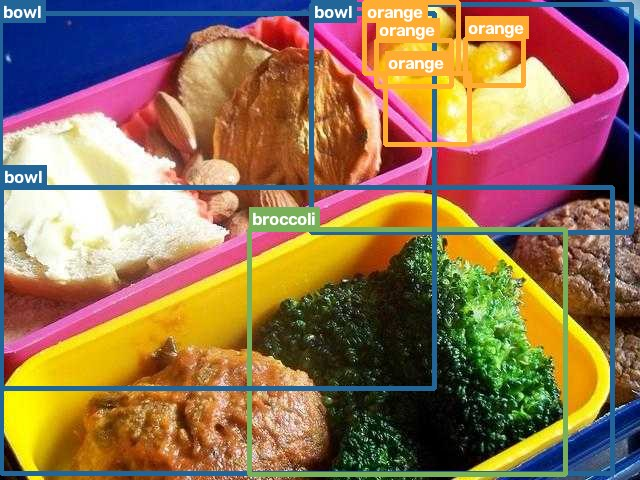
\includegraphics[height=0.72\textheight]{figures/yolo_coco_annotation.jpg}
\end{column}
\begin{column}{0.35\textwidth}
\begin{itemize}
  \item Bild \texttt{000000000009} aus \texttt{train2017}, $640 \times 480$ Pixel
  \item 8 Objekte aus 3 Klassen: 3-mal bowl, 4-mal orange, 1-mal broccoli
  \item Boxen \textbf{überlappen} stark, Schüsseln sind teilweise verdeckt.
  \item Labelzeile für broccoli: \texttt{50 0.637 0.733 0.494 0.511}
  \item Auch COCO ist \textbf{nicht fehlerfrei}: Die gelben Obststücke sind als orange annotiert, das Gebäck rechts gar nicht.
\end{itemize}
\end{column}
\end{columns}
\source{Bild und Annotationen: \cite{lin2014coco}, Teilmenge coco8 \cite{ultralytics_coco8}}
\end{frame}

% ---------------------------------------------------------
\begin{frame}[fragile]{Ultralytics: Installation und erste Vorhersage}
\footnotesize
\begin{columns}
\begin{column}{0.60\textwidth}
{\footnotesize
\begin{minted}{python}
# pip install ultralytics==8.4.215
from ultralytics import YOLO

model = YOLO("yolo26n.pt")    # lädt Gewichte
results = model.predict("bus.jpg", conf=0.25)
results[0].show()
\end{minted}
}
Alternativ über die Kommandozeile:
{\footnotesize
\begin{minted}{text}
yolo predict model=yolo26n.pt source=bus.jpg
\end{minted}
}
\end{column}
\begin{column}{0.35\textwidth}
\begin{itemize}
  \item Ultralytics basiert auf \textbf{PyTorch}, nicht auf Keras.
  \item Die High-Level-API verbirgt das Framework weitgehend.
  \item Gewichte werden beim ersten Aufruf \textbf{automatisch} geladen.
  \item Version festlegen, da sich das Paket schnell ändert
  \item Lizenz: \textbf{AGPL-3.0}, für kommerzielle Produkte ist eine Enterprise-Lizenz nötig.
\end{itemize}
\end{column}
\end{columns}
\source{\cite{ultralytics_predict}, \texttt{YoloAnwenden.ipynb}}
\end{frame}

% ---------------------------------------------------------
\begin{frame}{Ergebnis: YOLO26n auf einem Beispielbild}
\footnotesize
\begin{columns}
\begin{column}{0.35\textwidth}
\begin{itemize}
  \item Vortrainiert auf \textbf{COCO} mit 80 Alltagsklassen
  \item Gefunden: ein Bus und vier Personen
  \item Laufzeit auf einer CPU: rund 100\,ms pro Bild
  \item \texttt{r.plot()} zeichnet Boxen, Klassen und Confidence ein.
\end{itemize}
\end{column}
\begin{column}{0.60\textwidth}
\centering
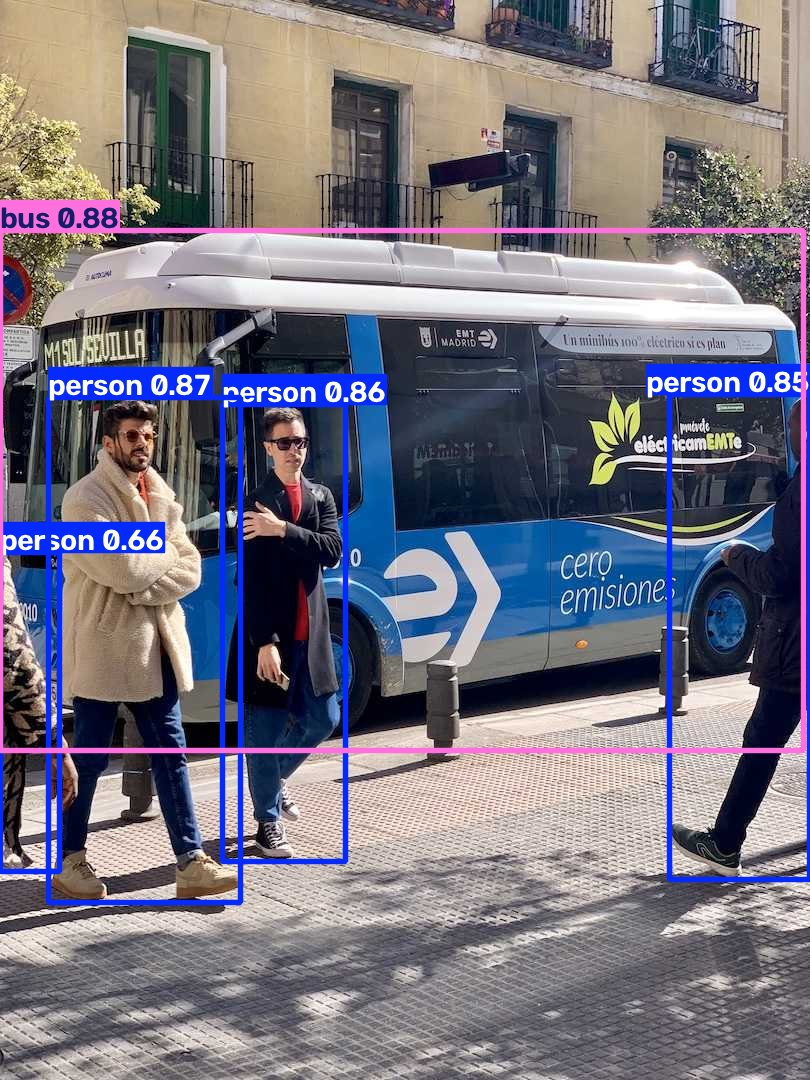
\includegraphics[height=0.72\textheight]{figures/yolo_bus.jpg}
\end{column}
\end{columns}
\source{Bildquelle: \cite{ultralytics_predict}}
\end{frame}

% ---------------------------------------------------------
\begin{frame}[fragile]{Das Results-Objekt}
\footnotesize
\begin{columns}
\begin{column}{0.47\textwidth}
{\footnotesize
\begin{minted}{python}
from collections import Counter

r = model.predict("bus.jpg")[0]
for box, c, k in zip(r.boxes.xyxy,
                     r.boxes.conf,
                     r.boxes.cls):
    print(r.names[int(k)], float(c),
          box.tolist())

Counter(r.names[int(k)]
        for k in r.boxes.cls)
\end{minted}
}
\end{column}
\begin{column}{0.48\textwidth}
\centering
\begin{tabular}{ll}
\toprule
\textbf{Attribut} & \textbf{Inhalt} \\
\midrule
\texttt{r.boxes.xyxy} & Boxen in Pixeln \\
\texttt{r.boxes.xywhn} & Boxen im YOLO-Format \\
\texttt{r.boxes.conf} & Confidence \\
\texttt{r.boxes.cls} & Klassen-IDs \\
\texttt{r.names} & ID $\rightarrow$ Klassenname \\
\texttt{r.speed} & Laufzeiten in ms \\
\texttt{r.plot()} & Bild mit Boxen \\
\bottomrule
\end{tabular}
\end{column}
\end{columns}
\source{\cite{ultralytics_predict}, \texttt{YoloAnwenden.ipynb} }
\end{frame}

% ---------------------------------------------------------
\begin{frame}[fragile]{Video, Webcam und Tracking}
\footnotesize
\begin{columns}
\begin{column}{0.60\textwidth}
{\footnotesize
\begin{minted}{python}
# Webcam mit Anzeigefenster
model.predict(source=0, show=True, conf=0.4)

# Frame für Frame verarbeiten
for r in model.predict(source=0, stream=True):
    print(len(r.boxes), "Objekte")

# Objekte über Frames hinweg verfolgen
for r in model.track(source="video.mp4",
                     stream=True, persist=True):
    print(r.boxes.id)
\end{minted}
}
\end{column}
\begin{column}{0.35\textwidth}
\begin{itemize}
  \item \texttt{source}: Bild, Ordner, Video, URL oder Kamera-Index
  \item \texttt{stream=True}: Generator, nicht alle Frames im Speicher
  \item \texttt{track}: Jedes Objekt behält über die Frames eine \textbf{ID}.
  \item Tracking erlaubt z.\,B. das Zählen von Objekten, die eine Linie überqueren.
\end{itemize}
\end{column}
\end{columns}
\source{\cite{ultralytics_predict}, \texttt{YoloAnwenden.ipynb}}
\end{frame}

% ---------------------------------------------------------
\begin{frame}{Warum erkennt YOLO26n keine Münzen?}
\footnotesize
\begin{columns}
\begin{column}{0.47\textwidth}
\begin{itemize}
  \item Das COCO-Modell findet auf dem Münzbild \textbf{nichts}, selbst bei \texttt{conf=0.1}.
  \item COCO enthält \textbf{keine Klasse für Münzen}.
  \item Ein Modell kann nur erkennen, was es gelernt hat.
  \item Der Backbone hat trotzdem nützliche Merkmale gelernt: Kanten, Kreise, Farben, Texturen.
\end{itemize}
\vfill
\textbf{Lösung: Transfer Learning} mit einem eigenen Münzdatensatz, wie bei VGG16 für Hunde und Katzen
\end{column}
\begin{column}{0.48\textwidth}
\centering
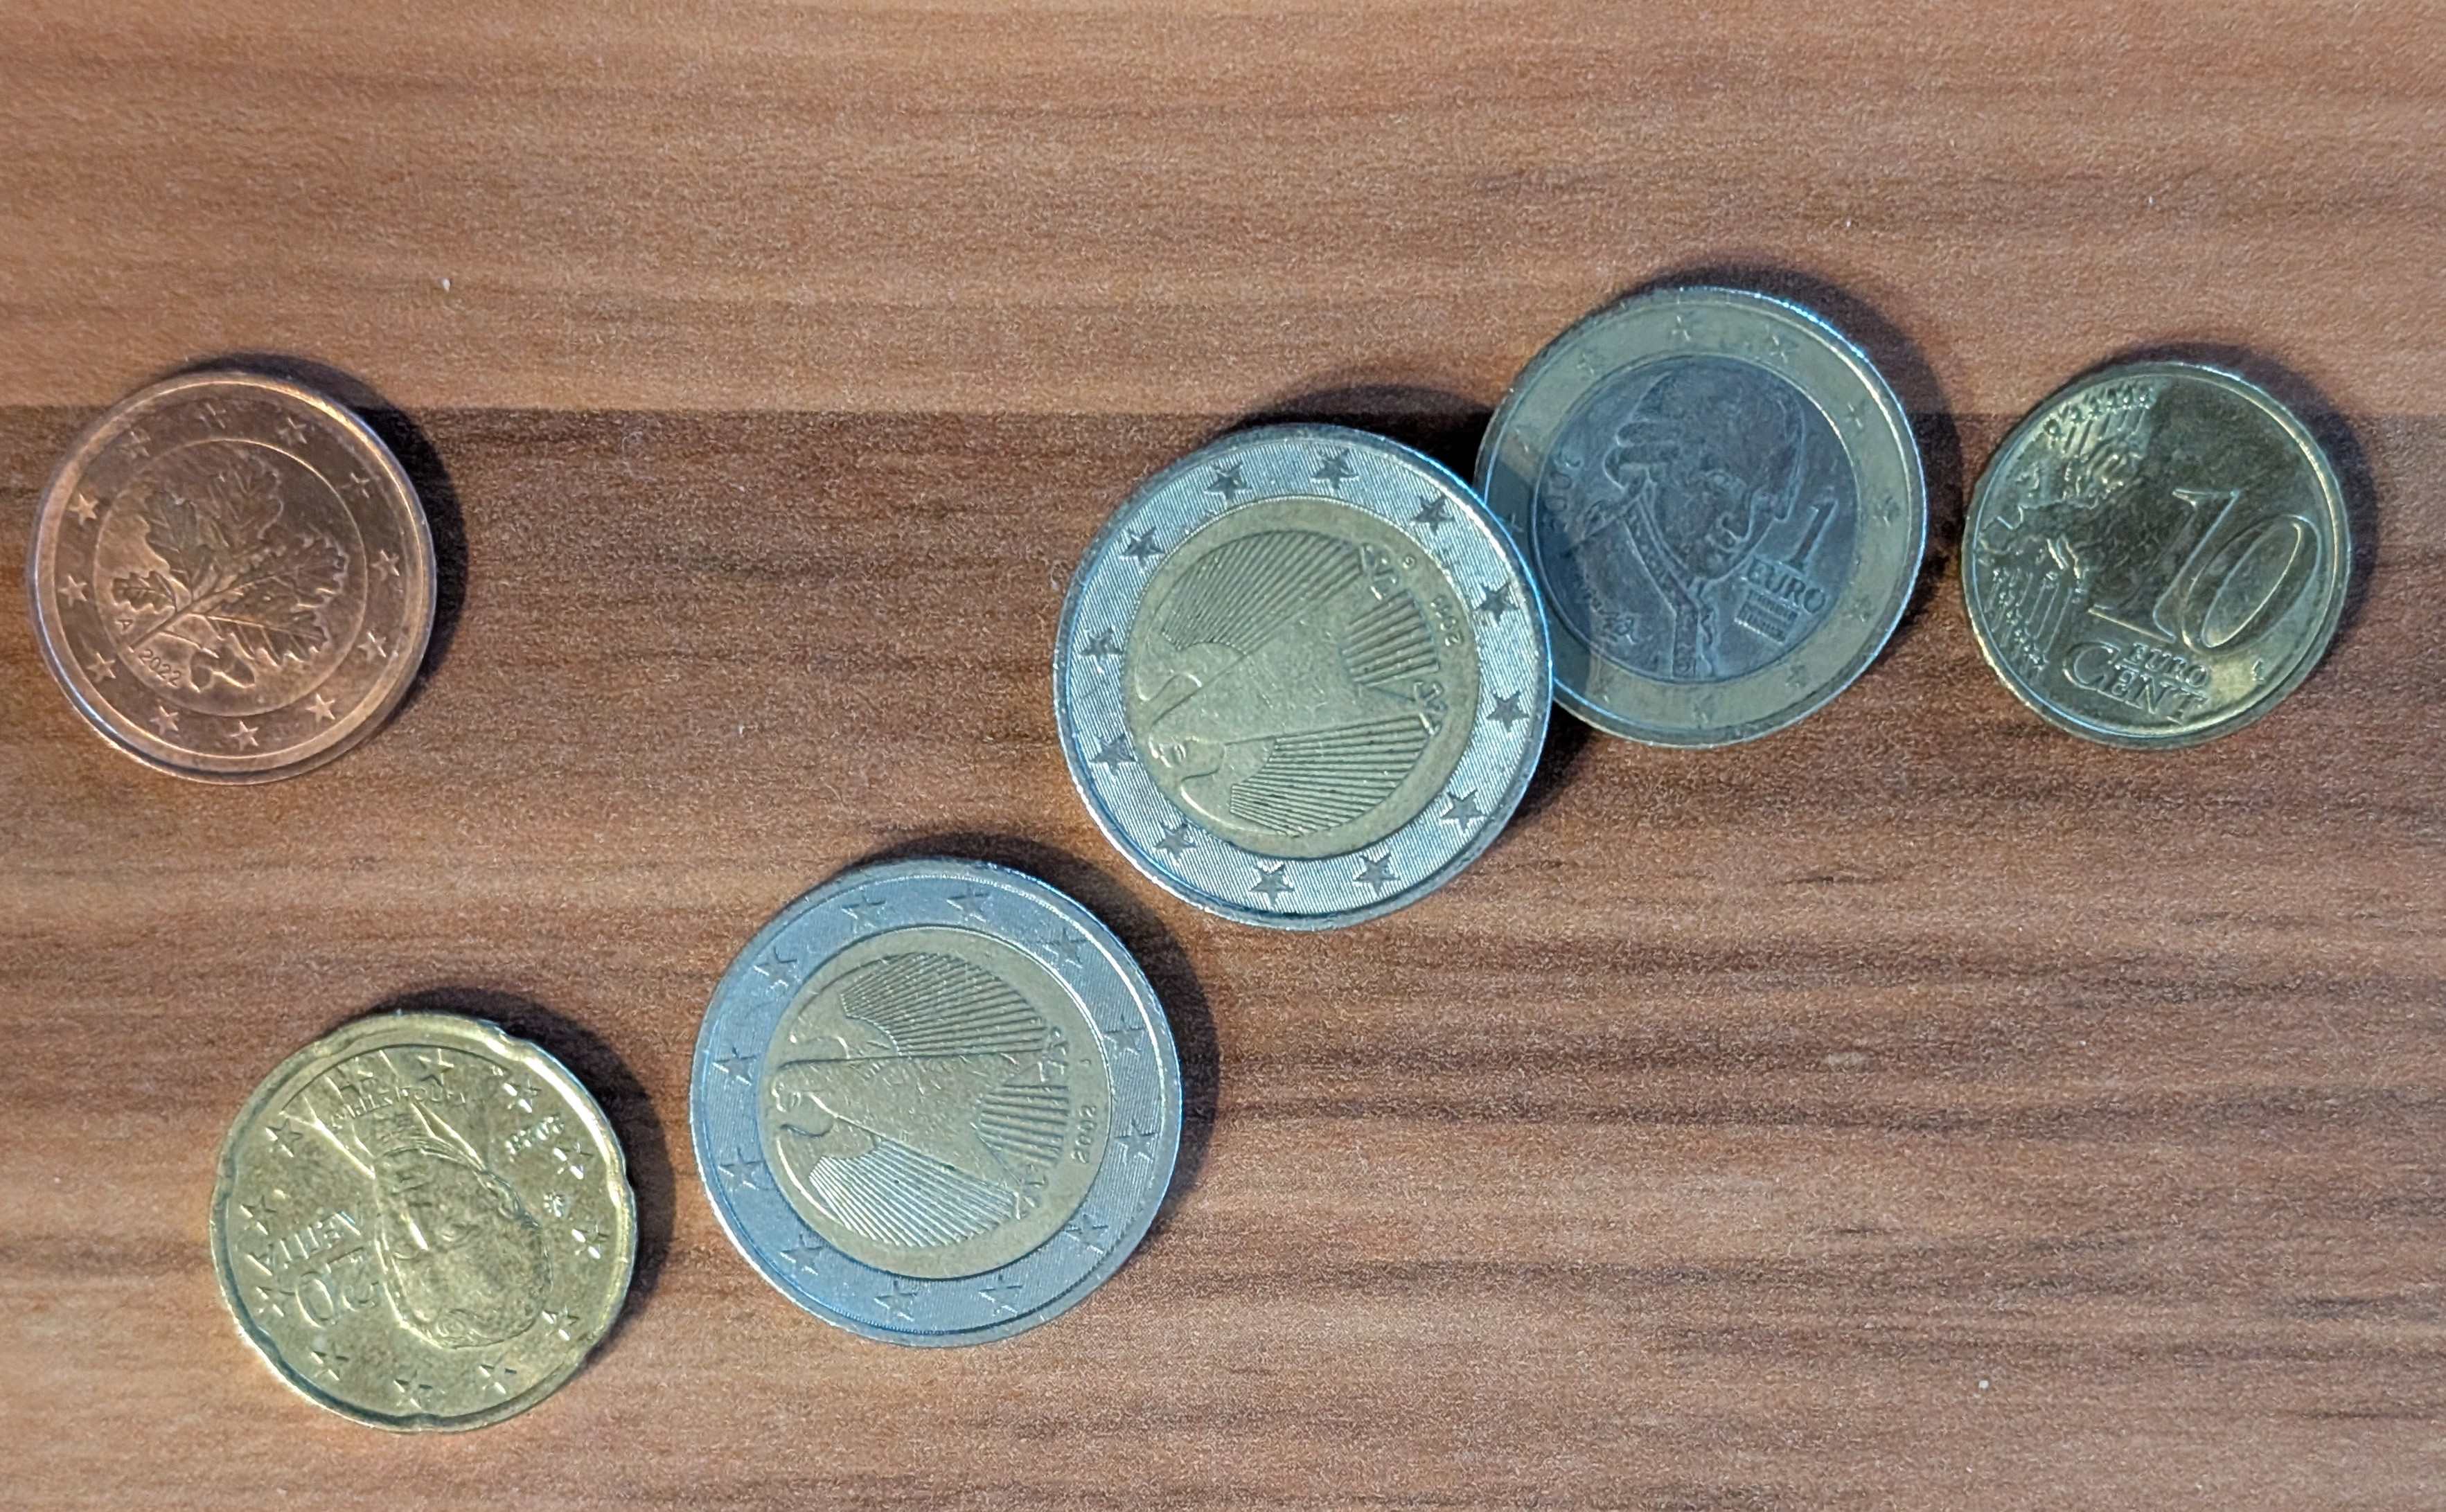
\includegraphics[width=0.9\linewidth]{figures/yolo_muenzen.jpg}
\end{column}
\end{columns}
\end{frame}

% ---------------------------------------------------------
\begin{frame}{Aufgabe: Vortrainiertes YOLO anwenden}
\footnotesize
\begin{columns}
\begin{column}{0.60\textwidth}
\begin{enumerate}
  \item Wenden Sie YOLO26n auf \texttt{strasse.jpg} und \texttt{bus.jpg} an und zählen Sie die Objekte je Klasse.
  \item Vergleichen Sie YOLO26n und YOLO26s hinsichtlich der Anzahl der Detektionen, der mittleren Confidence und der Laufzeit.
  \item Untersuchen Sie, wie die Anzahl erkannter Objekte vom Schwellenwert \texttt{conf} abhängt.
  \item Wenden Sie das vortrainierte Modell auf ein Münzbild an und erklären Sie das Ergebnis.
\end{enumerate}
\end{column}
\begin{column}{0.35\textwidth}
\centering
\twemoji[width=0.9\linewidth]{laptop}
\end{column}
\end{columns}
\source{Lösung: \texttt{LösungYoloAnwenden.ipynb}}
\end{frame}

\makesubsectionpage{Der Münzdatensatz}

% ---------------------------------------------------------
\begin{frame}{Woher kommen die Trainingsdaten?}
\footnotesize
\setbeamerfont{block title}{size=\footnotesize}
\begin{columns}
\begin{column}{0.60\textwidth}
\begin{blockrow}
  \begin{blockcol}{0.48\linewidth}{blockC1}{Eigene Daten}
    \begin{itemize}
      \item Fotos aufnehmen, annotieren, aufteilen
      \item Passt genau zur Anwendung.
      \item Aufwendig, vor allem das Annotieren
    \end{itemize}
  \end{blockcol}
  \begin{blockcol}{0.48\linewidth}{blockC2}{Öffentlicher Datensatz}
    \begin{itemize}
      \item Z.\,B. Roboflow Universe, Kaggle, Hochschulprojekte
      \item Sofort verfügbar
      \item Lizenz und Qualität müssen geprüft werden.
    \end{itemize}
  \end{blockcol}
\end{blockrow}
\end{column}
\begin{column}{0.35\textwidth}
\begin{itemize}
  \item In dieser Vorlesung: \textbf{öffentlicher Datensatz} als Grundlage
  \item Eigene Fotos dienen als \textbf{Live-Testset}.
  \item Die nächsten Folien zeigen, wie man eigene Daten aufnimmt und annotiert.
\end{itemize}
\end{column}
\end{columns}
\end{frame}

% ---------------------------------------------------------
\begin{frame}{Eigene Daten aufnehmen: Anforderungen}
\footnotesize
\begin{columns}
\begin{column}{0.60\textwidth}
\begin{itemize}
  \item \textbf{Umfang:} Für die Vorlesung reichen 200 bis 300 Bilder. Entscheidend ist die Zahl der \textbf{annotierten Münzen}, nicht der Bilder.
  \item \textbf{Viele Objekte pro Bild:} 5 bis 15 Münzen, auch überlappend
  \item \textbf{Variation} ist wichtiger als Menge:
  \begin{itemize}
    \item Untergrund, Licht und Tageszeit
    \item Vorder- und Rückseiten verschiedener Länder
    \item Abgegriffene und glänzende Münzen
    \item Verschiedene Kameras
  \end{itemize}
  \item \textbf{Hintergrundbilder} ohne Münzen, etwa 5 bis 10\,\%, gegen Fehlalarme
  \item \textbf{Feste Kamerahöhe}, damit die Größe als Merkmal nutzbar bleibt
\end{itemize}
\end{column}
\begin{column}{0.35\textwidth}
\centering
\twemoji[width=0.8\linewidth]{camera}
\end{column}
\end{columns}
\end{frame}

% ---------------------------------------------------------
\begin{frame}{Datenleck: Aufteilung nach Aufnahmeort}
\footnotesize
\begin{columns}
\begin{column}{0.47\textwidth}
\begin{itemize}
  \item Bilder einer Serie sind sich \textbf{fast identisch}.
  \item Zufällige Aufteilung bringt nahezu gleiche Bilder in Training und Validierung. Die mAP ist dann \textbf{zu optimistisch}.
  \item Daher \textbf{nach Aufnahmeort oder Sitzung} aufteilen
  \item Das Testset stammt aus einem Raum, der im Training nie vorkam.
  \item Dateinamen mit Ort als Präfix, z.\,B. \texttt{labor\_017.jpg}
\end{itemize}
\end{column}
\begin{column}{0.48\textwidth}
\centering
\resizebox{0.9\linewidth}{!}{%
\begin{tikzpicture}[
  ort/.style={draw, rounded corners=2pt, minimum width=1.9cm, minimum height=0.6cm, font=\small},
  pfeil/.style={-{Latex[length=2mm]}, line width=0.7pt, DarkGrey}]
  \node[ort, fill=SecondaryColor!20] (o1) at (0,2.4) {Hörsaal};
  \node[ort, fill=SecondaryColor!20] (o2) at (0,1.6) {Labor};
  \node[ort, fill=SecondaryColor!20] (o3) at (0,0.8) {Büro};
  \node[ort, fill=AccentColor!30] (o4) at (0,0) {Mensa};
  \node[ort, fill=ExampleColor!35] (o5) at (0,-0.8) {Bibliothek};
  \node[ort, fill=SecondaryColor!40, minimum height=1.9cm, minimum width=2.2cm] (tr) at (4,1.6) {\textbf{Training}};
  \node[ort, fill=AccentColor!50, minimum width=2.2cm] (va) at (4,0) {\textbf{Validierung}};
  \node[ort, fill=ExampleColor!55, minimum width=2.2cm] (te) at (4,-0.8) {\textbf{Test}};
  \foreach \o in {o1,o2,o3} \draw[pfeil] (\o.east) -- (tr.west);
  \draw[pfeil] (o4.east) -- (va.west);
  \draw[pfeil] (o5.east) -- (te.west);
\end{tikzpicture}%
}
\end{column}
\end{columns}
\end{frame}

% ---------------------------------------------------------
\begin{frame}[fragile]{COCO-Format und YOLO-Format}
\footnotesize
\begin{columns}
\begin{column}{0.60\textwidth}
{\footnotesize
\begin{minted}{json}
{
  "images": [
    {"id": 1, "file_name": "labor_017.jpg",
     "width": 1280, "height": 960}],
  "annotations": [
    {"id": 1, "image_id": 1, "category_id": 8,
     "bbox": [512, 384, 128, 128]}],
  "categories": [
    {"id": 8, "name": "2eur"}]
}
\end{minted}
}
Entspricht der YOLO-Zeile \texttt{7 0.450 0.467 0.100 0.133}
\end{column}
\begin{column}{0.35\textwidth}
\begin{itemize}
  \item COCO: \textbf{eine JSON-Datei} für den ganzen Datensatz
  \item \texttt{bbox}: $(x_1, y_1, w, h)$ in \textbf{Pixeln}
  \item Kategorie-IDs beginnen meist bei $1$.
  \item YOLO: eine Textdatei pro Bild, normiert, IDs ab $0$
  \item Viele Werkzeuge exportieren beide Formate.
  \item Umwandlung mit \texttt{convert\_coco()} aus \texttt{ultralytics.data.converter}
\end{itemize}
\end{column}
\end{columns}
\source{\cite{lin2014coco, ultralytics_datasets_detect}}
\end{frame}


% ---------------------------------------------------------
\begin{frame}{Annotationswerkzeuge}
\footnotesize
\begin{columns}
\begin{column}{0.60\textwidth}
\centering
\begin{tabular}{>{\raggedright\arraybackslash}p{2cm}>{\raggedright\arraybackslash}p{3.3cm}>{\raggedright\arraybackslash}p{3.3cm}}
\toprule
\textbf{Werkzeug} & \textbf{Vorteile} & \textbf{Nachteile} \\
\midrule
Label Studio & Lokal per \texttt{pip} installierbar, Daten bleiben auf dem Rechner & Gemeinsames Arbeiten nur mit Server \\
\midrule
CVAT & Open Source, Aufgaben auf Personen verteilbar, selbst hostbar & Betrieb aufwendig, sonst Cloud \\
\midrule
Roboflow & Sehr bequem, Aufteilung und Export integriert & Cloud-Dienst, Daten liegen extern \\
\bottomrule
\end{tabular}
\end{column}
\begin{column}{0.35\textwidth}
\begin{itemize}
  \item Alle drei exportieren direkt im \textbf{YOLO-Format}.
  \item Für die Lehre: CVAT über das Rechenzentrum oder Label Studio lokal
  \item Bei Fotos mit Personen auf den \textbf{Datenschutz} achten
\end{itemize}
\end{column}
\end{columns}
\end{frame}

% ---------------------------------------------------------
\begin{frame}{Annotationsrichtlinie}
\footnotesize
\setbeamerfont{block title}{size=\footnotesize}
\begin{columns}
\begin{column}{0.60\textwidth}
\begin{enumerate}
  \item Die Box liegt \textbf{eng} am Objekt an.
  \item \textbf{Jede} Münze im Bild wird annotiert.
  \item Bei Verdeckung wird nur der \textbf{sichtbare Teil} umrahmt.
  \item Münzen, die am Bildrand abgeschnitten sind, werden annotiert.
  \item Nicht mehr erkennbare Münzen werden nach einer \textbf{festen Regel} ausgelassen, z.\,B. kleiner als 15 Pixel.
  \item Jede Klasse hat eine Definition mit Beispielen und \textbf{Grenzfällen}.
\end{enumerate}
\end{column}
\begin{column}{0.35\textwidth}
\begin{blockC3}{Häufigster Fehler}
Eine vergessene Münze lernt das Modell als \textbf{Hintergrund}. Es wird dafür bestraft, sie zu erkennen.
\end{blockC3}
\vspace{0.5em}
Ohne gemeinsame Richtlinie annotiert jede Gruppe anders.
\end{column}
\end{columns}
\end{frame}

% ---------------------------------------------------------
\begin{frame}{Ablauf in der Gruppe und Vorannotation}
\footnotesize
\begin{columns}
\begin{column}{0.47\textwidth}
\begin{enumerate}
  \item Jede Gruppe fotografiert 30 bis 50 Bilder an \textbf{ihrem} Ort.
  \item Jede Gruppe annotiert die eigenen Bilder, etwa 10 bis 20 Sekunden pro Box.
  \item Eine andere Gruppe prüft rund 10\,\% der Bilder. Die \textbf{IoU} zwischen zwei Annotierenden misst die Übereinstimmung.
  \item Export im YOLO-Format, Aufteilung nach Ort
\end{enumerate}
\end{column}
\begin{column}{0.48\textwidth}
\begin{itemize}
  \item \textbf{Vorannotation:} Nach etwa 50 Bildern ein Nano-Modell trainieren
  \item Das Modell schlägt Boxen für die restlichen Bilder vor.
  \item Menschen \textbf{korrigieren} nur noch.
  \item Spart Zeit und zeigt, wie Datensätze in der Praxis wachsen
\end{itemize}
\vspace{0.5em}
\centering
\resizebox{0.8\linewidth}{!}{%
\begin{tikzpicture}[schritt/.style={draw, rounded corners=2pt, fill=SecondaryColor!20, font=\small, minimum width=2cm, minimum height=0.6cm}]
  \node[schritt] (a) at (0,1) {annotieren};
  \node[schritt] (b) at (3,1) {trainieren};
  \node[schritt] (c) at (3,0) {vorschlagen};
  \node[schritt] (d) at (0,0) {korrigieren};
  \draw[-{Latex[length=2mm]}, line width=0.7pt] (a) -- (b);
  \draw[-{Latex[length=2mm]}, line width=0.7pt] (b) -- (c);
  \draw[-{Latex[length=2mm]}, line width=0.7pt] (c) -- (d);
  \draw[-{Latex[length=2mm]}, line width=0.7pt] (d) -- (a);
\end{tikzpicture}%
}
\end{column}
\end{columns}
\end{frame}

% ---------------------------------------------------------
\begin{frame}{Unser Datensatz von Roboflow Universe}
\footnotesize
\begin{columns}
\begin{column}{0.47\textwidth}
\begin{itemize}
  \item „Small object detection for euro coins“, Version 5 von 2023
  \item Lizenz: \textbf{Public Domain}
  \item \textbf{1789 Bilder} mit $512 \times 512$ Pixeln
  \item \textbf{8 Klassen}: 1, 2, 5, 10, 20 und 50 Cent sowie 1\,€ und 2\,€
  \item Münzen von oben fotografiert, verschiedene Untergründe, Abstände und Länderseiten
  \item In dieser Version keine Vorverarbeitung und keine Augmentierung
\end{itemize}
\end{column}
\begin{column}{0.48\textwidth}
\centering
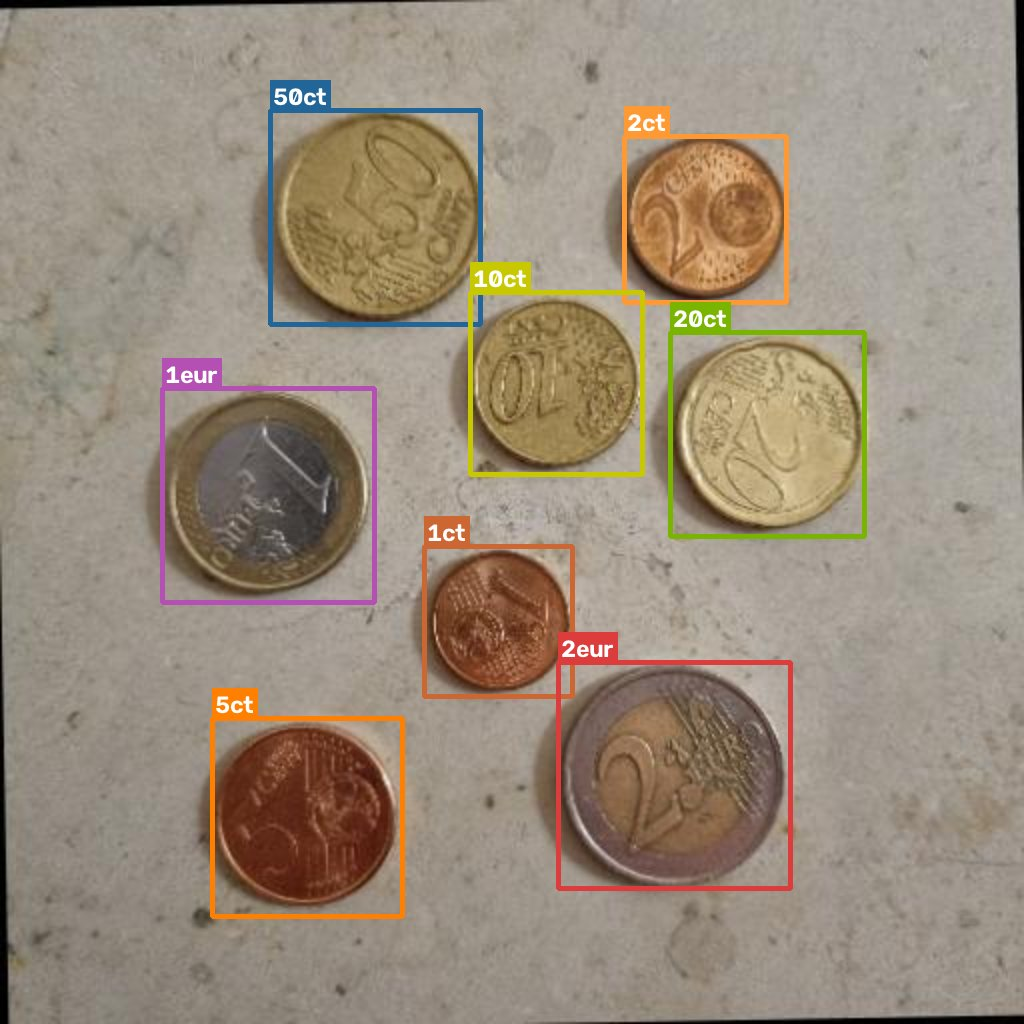
\includegraphics[width=0.9\linewidth]{figures/yolo_datensatz_beispiel.jpg}
\end{column}
\end{columns}
\source{Datensatz und Bild: \cite{hlcv2023coins}, Boxen neu eingezeichnet}
\end{frame}

% ---------------------------------------------------------
\begin{frame}{Öffentliche Datensätze kritisch prüfen}
\footnotesize
\setbeamerfont{block title}{size=\footnotesize}
\begin{columns}
\begin{column}{0.47\textwidth}
\begin{blockC3}{Erfahrung mit einem anderen Münzdatensatz}
\begin{itemize}
  \item Klassennamen waren Textzeilen aus einer README.
  \item Münzen und Geldscheine gemischt
  \item Dieselbe Münze unter mehreren Klassen-IDs
\end{itemize}
\end{blockC3}
\textbf{Prüfliste vor dem Training:}
\begin{itemize}
  \item Lizenz, Quelle und Klassennamen
  \item Ausschnitte je Klasse ansehen
  \item Duplikate und Überschneidungen der Splits
\end{itemize}
\end{column}
\begin{column}{0.48\textwidth}
\centering
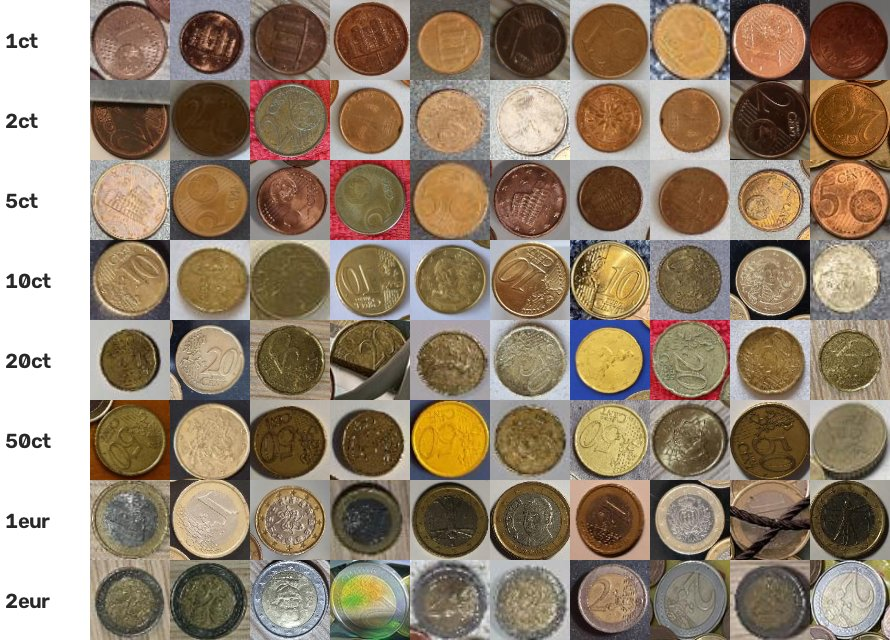
\includegraphics[width=0.9\linewidth]{figures/yolo_klassen_uebersicht.jpg}

\scriptsize Ausschnitte je Klasse aus unserem Datensatz
\end{column}
\end{columns}
\source{Bilder: \cite{hlcv2023coins}}
\end{frame}

% ---------------------------------------------------------
\begin{frame}{Datensatz reduzieren}
\footnotesize
\begin{columns}
\begin{column}{0.47\textwidth}
\begin{itemize}
  \item Viele Trainingsbilder liegen \textbf{dreifach} vor: augmentierte Kopien aus früheren Versionen, erkennbar am gleichen Namen vor \texttt{.rf.}
  \item Ultralytics augmentiert selbst, die Kopien kosten nur Rechenzeit.
  \item Wir behalten \textbf{ein Bild pro Quellbild}.
  \item Klassen-IDs werden in die Reihenfolge der Vorlesung umnummeriert.
\end{itemize}
\vspace{0.5em}
\centering
\begin{tabular}{lrr}
\toprule
\textbf{Split} & \textbf{Roboflow} & \textbf{reduziert} \\
\midrule
Training & 1311 & 512 \\
Validierung & 146 & 146 \\
Test & 122 & 90 \\
\midrule
\textbf{Summe} & \textbf{1579} & \textbf{748} \\
\bottomrule
\end{tabular}
\end{column}
\begin{column}{0.48\textwidth}
\centering
\begin{tabular}{lcc}
\toprule
\textbf{Roboflow-Klasse} & \textbf{alt} & \textbf{neu} \\
\midrule
\texttt{EUR-1-cent} & 0 & 0 \\
\texttt{EUR-1-euro} & 1 & 6 \\
\texttt{EUR-10-cent} & 2 & 3 \\
\texttt{EUR-2-cent} & 3 & 1 \\
\texttt{EUR-2-euro} & 4 & 7 \\
\texttt{EUR-20-cent} & 5 & 4 \\
\texttt{EUR-5-cent} & 6 & 2 \\
\texttt{EUR-50-cent} & 7 & 5 \\
\bottomrule
\end{tabular}

\vspace{0.5em}
Ergebnis: Ordner \texttt{muenzen\_klein} mit 33\,MB statt 76\,MB
\end{column}
\end{columns}
\source{\cite{hlcv2023coins}}
\end{frame}

% ---------------------------------------------------------
\begin{frame}[fragile]{Verzeichnisstruktur und data.yaml}
\footnotesize
\begin{columns}
\begin{column}{0.47\textwidth}
{\footnotesize
\begin{minted}{text}
muenzen_klein/
  data.yaml
  images/
    train/  20210321_094710_jpg.jpg
    val/
    test/
  labels/
    train/  20210321_094710_jpg.txt
    val/
    test/
\end{minted}
}
\begin{itemize}
  \item Labels liegen im parallelen Ordner \texttt{labels}.
  \item Ohne \texttt{path} gelten die Pfade relativ zur \texttt{data.yaml}.
\end{itemize}
\end{column}
\begin{column}{0.48\textwidth}
{\footnotesize
\begin{minted}{yaml}
train: images/train
val: images/val
test: images/test

names:
  0: 1ct
  1: 2ct
  2: 5ct
  3: 10ct
  4: 20ct
  5: 50ct
  6: 1eur
  7: 2eur
\end{minted}
}
\end{column}
\end{columns}
\source{\cite{ultralytics_datasets_detect}}
\end{frame}

% ---------------------------------------------------------
\begin{frame}{Labels prüfen}
\footnotesize
\begin{columns}
\begin{column}{0.60\textwidth}
\begin{itemize}
  \item \textbf{Plausibilität:} Klassen-IDs zwischen $0$ und $7$, alle Koordinaten in $[0, 1]$
  \item \textbf{Klassenverteilung:} Gibt es genug 1-ct- und 20-ct-Münzen?
  \item \textbf{Boxgrößen:} Passen sie zur Kamerahöhe?
  \item \textbf{Sichtprüfung:} Boxen auf Stichproben einzeichnen
  \item \textbf{Klassennamen:} Stimmt die Reihenfolge in \texttt{data.yaml} mit dem Export überein?
  \item Unser Trainingssplit: 3666 Münzen auf 473 Bildern, dazu 39 Hintergrundbilder
\end{itemize}
\vspace{0.5em}
Fehler im Datensatz lassen sich durch kein Training ausgleichen.
\end{column}
\begin{column}{0.35\textwidth}
\centering
\twemoji[width=0.8\linewidth]{mag}
\end{column}
\end{columns}
\end{frame}

% ---------------------------------------------------------
\begin{frame}{Aufgabe: Münzdatensatz vorbereiten}
\footnotesize
\begin{columns}
\begin{column}{0.60\textwidth}
\begin{enumerate}
  \item Laden Sie den Datensatz „Small object detection for euro coins“ (Version 5) im Format YOLOv8 von Roboflow Universe herunter.
  \item Erzeugen Sie den reduzierten Datensatz mit einem Bild pro Quellbild und den Klassen-IDs der Vorlesung.
  \item Prüfen Sie Klassenverteilung und Boxgrößen und sehen Sie sich Ausschnitte je Klasse an. Finden Sie falsch annotierte Münzen?
  \item Optional: Fotografieren und annotieren Sie 30 bis 50 eigene Münzbilder als Live-Testset.
\end{enumerate}
\end{column}
\begin{column}{0.35\textwidth}
\centering
\twemoji[width=0.9\linewidth]{laptop}
\end{column}
\end{columns}
\source{Lösung: \texttt{LösungDatensatzVorbereiten.ipynb}}
\end{frame}

\makesubsectionpage{Training}

% ---------------------------------------------------------
\begin{frame}{Transfer Learning mit YOLO}
\footnotesize
\setbeamerfont{block title}{size=\footnotesize}
\begin{columns}
\begin{column}{0.47\textwidth}
\begin{itemize}
  \item Ausgangspunkt sind die auf COCO \textbf{vortrainierten Gewichte}.
  \item Der Head wird automatisch auf \textbf{8 Klassen} umgebaut.
  \item Standardmäßig werden \textbf{alle Schichten} weitertrainiert.
  \item Mit \texttt{freeze=10} bleiben die ersten 10 Schichten fest, ähnlich zu \texttt{trainable = False} bei VGG16.
  \item Münzen unterscheiden sich stark von COCO. Vollständiges Fine-Tuning ist daher meist besser.
\end{itemize}
\end{column}
\begin{column}{0.48\textwidth}
\begin{blockrow}
  \begin{blockcol}{0.48\linewidth}{blockC1}{Keras mit VGG16}
    \begin{itemize}
      \item Basis laden ohne Top
      \item Eigene Dense-Layer anhängen
      \item Basis einfrieren
      \item \texttt{model.fit()}
    \end{itemize}
  \end{blockcol}
  \begin{blockcol}{0.48\linewidth}{blockC2}{Ultralytics}
    \begin{itemize}
      \item Vortrainiertes Modell laden
      \item Head passt sich an \texttt{data.yaml} an.
      \item Optional \texttt{freeze}
      \item \texttt{model.train()}
    \end{itemize}
  \end{blockcol}
\end{blockrow}
\end{column}
\end{columns}
\source{\cite{ultralytics_train}}
\end{frame}

% ---------------------------------------------------------
\begin{frame}[fragile]{Training starten}
\footnotesize
\begin{columns}
\begin{column}{0.47\textwidth}
{\footnotesize
\begin{minted}{python}
from ultralytics import YOLO

model = YOLO("yolo26n.pt")
results = model.train(
    data="muenzen/data.yaml",
    epochs=50,
    imgsz=640,
    batch=16,
    patience=10,
    name="muenzen",
)
\end{minted}
}
\end{column}
\begin{column}{0.48\textwidth}
\centering
\begin{tabular}{lrl}
\toprule
\textbf{Parameter} & \textbf{Standard} & \textbf{Bedeutung} \\
\midrule
\texttt{epochs} & 100 & Durchläufe \\
\texttt{patience} & 100 & Early Stopping \\
\texttt{batch} & 16 & Bilder pro Batch \\
\texttt{imgsz} & 640 & Eingabegröße \\
\texttt{lr0} & 0,01 & Lernrate \\
\texttt{optimizer} & \texttt{auto} & Optimierer \\
\texttt{freeze} & -- & Eingefrorene Schichten \\
\texttt{device} & auto & GPU oder CPU \\
\bottomrule
\end{tabular}
\end{column}
\end{columns}
\source{\cite{ultralytics_train}}
\end{frame}

% ---------------------------------------------------------
\begin{frame}{Augmentierung}
\footnotesize
\begin{columns}
\begin{column}{0.47\textwidth}
\begin{itemize}
  \item Ultralytics verändert die Trainingsbilder \textbf{zufällig} in jeder Epoche.
  \item \textbf{Mosaic:} vier Bilder zu einem kombiniert, in den letzten 10 Epochen abgeschaltet (\texttt{close\_mosaic})
  \item Spiegeln (\texttt{fliplr=0.5}), Farbe (\texttt{hsv\_h}, \texttt{hsv\_s}, \texttt{hsv\_v}), Verschieben und Skalieren
  \item \textbf{Achtung bei Münzen:} \texttt{scale=0.5} skaliert um bis zu $\pm 50\,\%$ und zerstört damit das Größenmerkmal. Bei fester Kamerahöhe besser \texttt{scale=0.1}.
  \item Augmentierung muss zur \textbf{Anwendung} passen.
\end{itemize}
\end{column}
\begin{column}{0.48\textwidth}
\centering
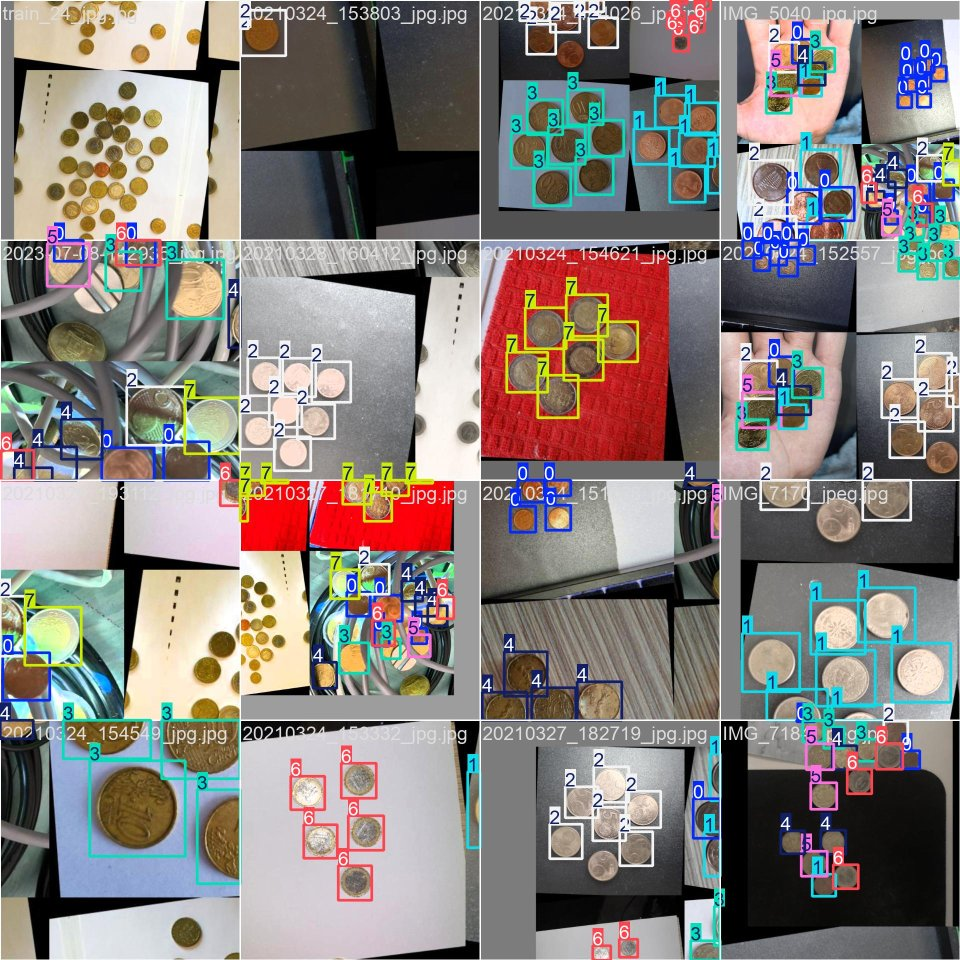
\includegraphics[width=0.9\linewidth]{figures/yolo_train_batch.jpg}

\scriptsize Trainingsbatch mit Mosaic-Augmentierung
\end{column}
\end{columns}
\source{\cite{ultralytics_train}}
\end{frame}

% ---------------------------------------------------------
\begin{frame}{Ergebnisse im Ordner runs/detect}
\footnotesize
\begin{columns}
\begin{column}{0.35\textwidth}
\begin{itemize}
  \item \texttt{weights/best.pt}: bestes Modell auf den Validierungsdaten
  \item \texttt{weights/last.pt}: letzter Stand, zum Fortsetzen
  \item \texttt{results.csv}, \texttt{results.png}: Verlauf
  \item \texttt{labels.jpg}: Klassen und Boxgrößen
  \item \texttt{train\_batch*.jpg}: augmentierte Batches
  \item \texttt{val\_batch*\_pred.jpg}: Vorhersagen
  \item \texttt{confusion\_matrix.png}
\end{itemize}
\end{column}
\begin{column}{0.60\textwidth}
\centering
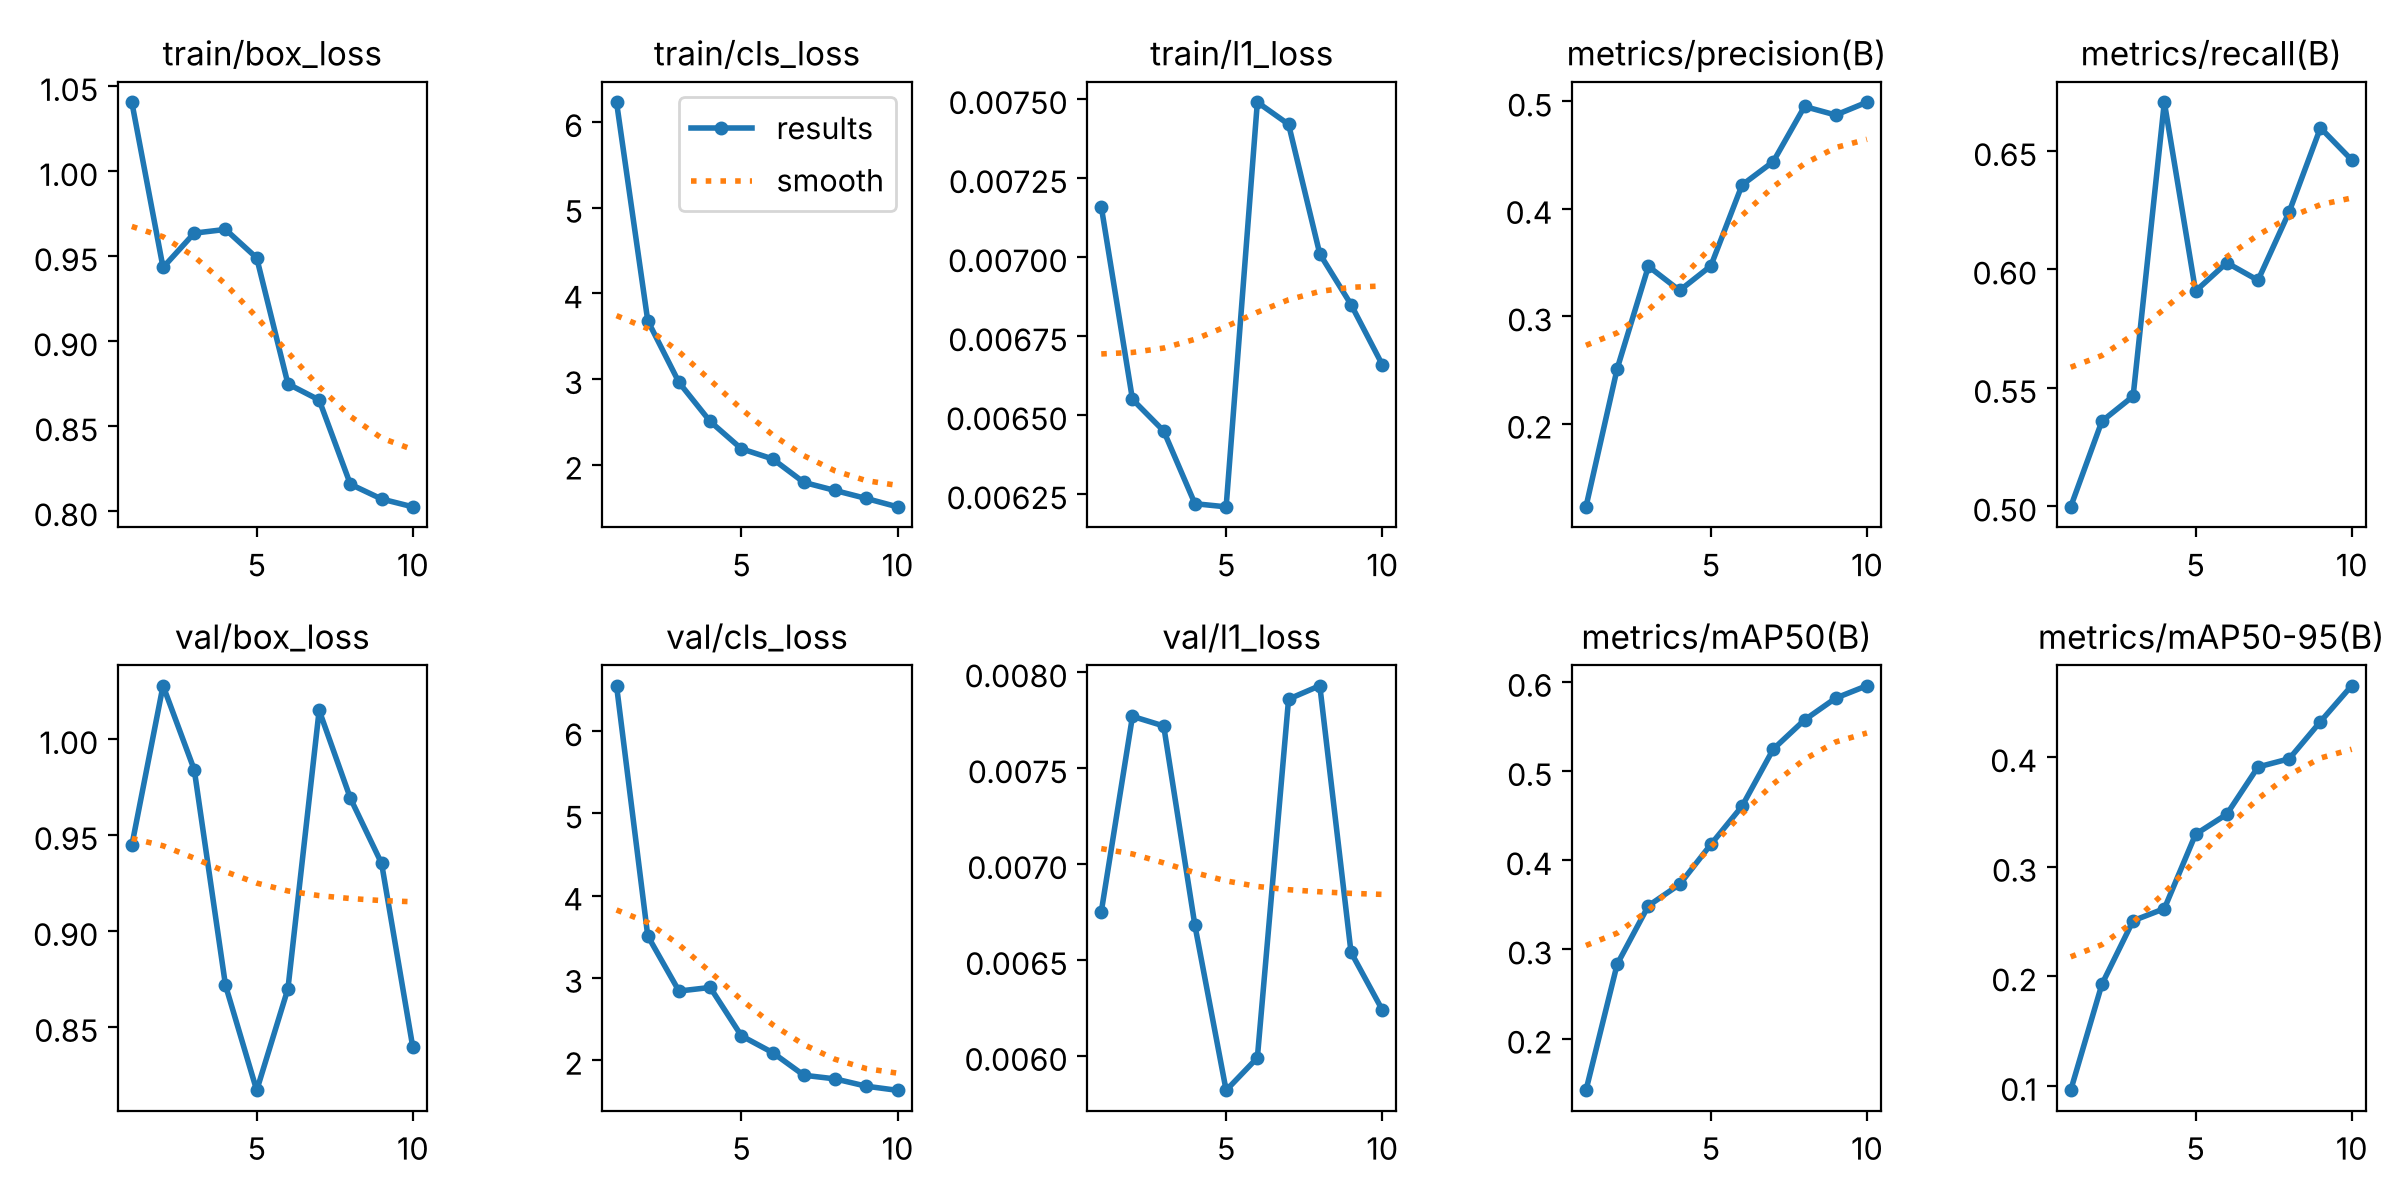
\includegraphics[width=0.95\linewidth]{figures/yolo_results.png}

\scriptsize Verlauf beim Training auf dem Münzdatensatz, 10 Epochen
\end{column}
\end{columns}
\end{frame}

% ---------------------------------------------------------
\begin{frame}{Trainingsverlauf lesen}
\footnotesize
\setbeamerfont{block title}{size=\footnotesize}
\begin{columns}
\begin{column}{0.47\textwidth}
\begin{itemize}
  \item Trainings- und Validierungs-Loss sollten \textbf{sinken}.
  \item Die mAP auf den Validierungsdaten sollte \textbf{steigen}.
  \item Steigt der Validierungs-Loss wieder, während der Trainings-Loss sinkt: \textbf{Overfitting}
  \item \texttt{patience}: Training endet, wenn sich die Validierungsgüte so viele Epochen nicht verbessert.
  \item \texttt{best.pt} enthält automatisch den besten Stand.
\end{itemize}
\end{column}
\begin{column}{0.48\textwidth}
\begin{blockC1}{Bekannt aus dem CNN-Kapitel}
\begin{itemize}
  \item Early Stopping mit \texttt{patience}
  \item \texttt{restore\_best\_weights} entspricht \texttt{best.pt}.
  \item Trainings- gegen Validierungskurve vergleichen
\end{itemize}
\end{blockC1}
\begin{blockC2}{Typische Ursachen schlechter Ergebnisse}
\begin{itemize}
  \item Zu wenige oder zu ähnliche Bilder
  \item Fehlerhafte oder vergessene Labels
  \item Unpassende Augmentierung
\end{itemize}
\end{blockC2}
\end{column}
\end{columns}
\end{frame}

% ---------------------------------------------------------
\begin{frame}{Hardware und Trainingszeit}
\footnotesize
\begin{columns}
\begin{column}{0.60\textwidth}
\begin{itemize}
  \item Unser Test: YOLO26n, 512 Trainingsbilder, $640 \times 640$ Pixel, CPU mit 2 Kernen
  \begin{itemize}
    \item Etwa \textbf{4,5 Minuten pro Epoche}, rund 6\,GB Arbeitsspeicher bei \texttt{batch=16}
    \item 50 Epochen dauern damit fast vier Stunden.
  \end{itemize}
  \item Mit einer GPU, z.\,B. in Google Colab, geht es um ein \textbf{Vielfaches} schneller.
  \item Stellschrauben bei wenig Rechenleistung:
  \begin{itemize}
    \item Kleineres Modell (\texttt{n} statt \texttt{s})
    \item Kleinere Eingabegröße, aber Vorsicht bei kleinen Münzen
    \item \texttt{batch=8} bei wenig Arbeitsspeicher
    \item Weniger Epochen mit \texttt{patience}
  \end{itemize}
\end{itemize}
\end{column}
\begin{column}{0.35\textwidth}
\centering
\twemoji[width=0.8\linewidth]{stopwatch}
\end{column}
\end{columns}
\end{frame}

% ---------------------------------------------------------
\begin{frame}{Aufgabe: YOLO26 auf Münzen trainieren}
\footnotesize
\begin{columns}
\begin{column}{0.60\textwidth}
\begin{enumerate}
  \item Trainieren Sie YOLO26n auf dem reduzierten Münzdatensatz.
  \item Stellen Sie Loss und mAP über die Epochen dar und beurteilen Sie, ob Overfitting auftritt.
  \item Sehen Sie sich \texttt{labels.jpg} und \texttt{train\_batch0.jpg} an. Was fällt Ihnen auf?
  \item Trainieren Sie mit \texttt{scale=0.1} statt des Standardwerts und vergleichen Sie die mAP.
  \item Optional: Vergleichen Sie Training mit vortrainierten Gewichten und Training von Null (\texttt{yolo26n.yaml}).
\end{enumerate}
\end{column}
\begin{column}{0.35\textwidth}
\centering
\twemoji[width=0.9\linewidth]{laptop}
\end{column}
\end{columns}
\source{Lösung: \texttt{LösungYoloTraining.ipynb}}
\end{frame}

\makesubsectionpage{Bewertung}

% ---------------------------------------------------------
\begin{frame}{Wann ist eine Detektion richtig?}
\footnotesize
\begin{columns}
\begin{column}{0.60\textwidth}
\begin{itemize}
  \item Detektionen werden absteigend nach Confidence den echten Objekten zugeordnet.
  \item \textbf{True Positive (TP):} richtige Klasse und $\operatorname{IoU} \geq$ Schwelle zu einem noch nicht zugeordneten Objekt
  \item \textbf{False Positive (FP):} falsche Klasse, zu geringe IoU oder Objekt schon zugeordnet
  \item \textbf{False Negative (FN):} echtes Objekt ohne passende Detektion
  \item \textbf{True Negatives} gibt es praktisch nicht: Die Zahl der „richtig leeren“ Boxen ist unbegrenzt.
  \item Daher keine Accuracy, sondern \textbf{Precision} und \textbf{Recall}
\end{itemize}
\end{column}
\begin{column}{0.35\textwidth}
\centering
\resizebox{0.9\linewidth}{!}{%
\begin{tikzpicture}
  \fill[DarkGrey!8] (0,0) rectangle (4,4);
  \yoloMuenze{(1.1,2.9)}{0.6}{SilberColor}{GoldColor}{2\,€}
  \yoloMuenze{(2.9,2.9)}{0.55}{GoldColor}{GoldColor}{50\,ct}
  \yoloMuenze{(1.2,1.0)}{0.45}{KupferColor}{KupferColor}{1\,ct}
  \draw[ExampleColor, line width=1.2pt] (0.45,2.25) rectangle (1.75,3.55);
  \node[font=\scriptsize\bfseries, ExampleColor!80!black, anchor=south] at (1.1,3.55) {TP};
  \draw[AlertColor, line width=1.2pt] (2.65,2.2) rectangle (3.75,3.3);
  \node[font=\scriptsize\bfseries, AlertColor, anchor=south] at (3.2,3.3) {FP};
  \draw[AlertColor, line width=1.2pt, dashed] (2.4,0.4) rectangle (3.6,1.6);
  \node[font=\scriptsize\bfseries, AlertColor, anchor=north] at (3.0,0.4) {FP};
  \node[font=\scriptsize\bfseries, AccentColor!80!black, anchor=north] at (1.2,0.5) {FN};
\end{tikzpicture}%
}
\end{column}
\end{columns}
\end{frame}

% ---------------------------------------------------------
\begin{frame}{Precision und Recall}
\footnotesize
\setbeamerfont{block title}{size=\footnotesize}
\begin{columns}
\begin{column}{0.47\textwidth}
\begin{definition}[Precision und Recall\strut]
\[
\text{Precision} = \frac{TP}{TP + FP}, \qquad
\text{Recall} = \frac{TP}{TP + FN}
\]
\end{definition}
\begin{itemize}
  \item \textbf{Precision:} Wie viele Detektionen sind richtig?
  \item \textbf{Recall:} Wie viele Münzen werden gefunden?
\end{itemize}
\end{column}
\begin{column}{0.48\textwidth}
\begin{itemize}
  \item Beide hängen vom Schwellenwert \texttt{conf} ab:
  \begin{itemize}
    \item Hoher Schwellenwert: hohe Precision, niedriger Recall
    \item Niedriger Schwellenwert: niedrige Precision, hoher Recall
  \end{itemize}
  \item Die \textbf{Precision-Recall-Kurve} zeigt alle Schwellenwerte auf einmal.
  \item Die Fläche darunter ist die \textbf{Average Precision (AP)}.
\end{itemize}
\end{column}
\end{columns}
\end{frame}

% ---------------------------------------------------------
\begin{frame}{Beispiel: Precision und Recall für die Klasse 1\,€}
\footnotesize
\begin{columns}
\begin{column}{0.60\textwidth}
\centering
\begin{tabular}{rcccc}
\toprule
\textbf{Conf.} & \textbf{TP/FP} & \textbf{kum. TP} & \textbf{Precision} & \textbf{Recall} \\
\midrule
0,95 & TP & 1 & 1,000 & 0,2 \\
0,91 & TP & 2 & 1,000 & 0,4 \\
0,85 & FP & 2 & 0,667 & 0,4 \\
0,80 & TP & 3 & 0,750 & 0,6 \\
0,72 & TP & 4 & 0,800 & 0,8 \\
0,60 & FP & 4 & 0,667 & 0,8 \\
0,45 & FP & 4 & 0,571 & 0,8 \\
0,30 & TP & 5 & 0,625 & 1,0 \\
\bottomrule
\end{tabular}
\end{column}
\begin{column}{0.35\textwidth}
\begin{itemize}
  \item 5 echte 1-€-Münzen in den Testbildern
  \item 8 Detektionen, absteigend nach Confidence sortiert
  \item Jede Zeile entspricht einem möglichen Schwellenwert.
  \item Precision $= \frac{\text{kum. TP}}{\text{Zeile}}$, Recall $= \frac{\text{kum. TP}}{5}$
\end{itemize}
\end{column}
\end{columns}
\end{frame}

% ---------------------------------------------------------
\begin{frame}{Average Precision}
\footnotesize
\setbeamerfont{block title}{size=\footnotesize}
\begin{columns}
\begin{column}{0.47\textwidth}
\begin{itemize}
  \item \textbf{Interpolation:} Für jeden Recall wird die höchste Precision bei gleichem oder höherem Recall verwendet.
  \item AP ist die Fläche unter der interpolierten Kurve.
\end{itemize}
\begin{beispiel}[AP für die Klasse 1\,€\strut]
\[
\begin{aligned}
AP &= 0{,}2 \cdot 1 + 0{,}2 \cdot 1 + 0{,}2 \cdot 0{,}8 \\
   &\quad + 0{,}2 \cdot 0{,}8 + 0{,}2 \cdot 0{,}625 \\
   &= 0{,}845
\end{aligned}
\]
\end{beispiel}
\end{column}
\begin{column}{0.48\textwidth}
\centering
\resizebox{0.9\linewidth}{!}{%
\begin{tikzpicture}
\begin{axis}[
  width=7cm, height=5.5cm,
  xmin=0, xmax=1.05, ymin=0, ymax=1.1,
  xlabel={Recall}, ylabel={Precision},
  grid=major, grid style={gray!25},
  tick label style={font=\footnotesize},
  legend style={font=\footnotesize, at={(0.03,0.03)}, anchor=south west}]
\addplot[fill=SecondaryColor!25, draw=none, const plot mark right, forget plot]
  coordinates {(0,1) (0.2,1) (0.4,1) (0.6,0.8) (0.8,0.8) (1.0,0.625)} \closedcycle;
\addplot[PrimaryColor, line width=1.2pt, const plot mark right]
  coordinates {(0,1) (0.2,1) (0.4,1) (0.6,0.8) (0.8,0.8) (1.0,0.625)};
\addplot[AlertColor, mark=*, only marks, mark size=1.8pt]
  coordinates {(0.2,1) (0.4,1) (0.4,0.667) (0.6,0.75) (0.8,0.8) (0.8,0.667) (0.8,0.571) (1.0,0.625)};
\legend{interpoliert, Messpunkte}
\end{axis}
\end{tikzpicture}%
}
\end{column}
\end{columns}
\end{frame}

% ---------------------------------------------------------
\begin{frame}{mAP@0.5 und mAP@0.5:0.95}
\footnotesize
\setbeamerfont{block title}{size=\footnotesize}
\begin{columns}
\begin{column}{0.60\textwidth}
\begin{definition}[Mean Average Precision\strut]
Für $K$ Klassen und eine IoU-Schwelle $t$ ist
\[
\text{mAP}@t = \frac{1}{K} \sum_{k=1}^{K} AP_k(t).
\]
Die COCO-Metrik mittelt zusätzlich über zehn Schwellen:
\[
\text{mAP}@0.5{:}0.95 = \frac{1}{10} \sum_{t \in \{0{,}50;\, 0{,}55;\, \dots;\, 0{,}95\}} \text{mAP}@t
\]
\end{definition}
\end{column}
\begin{column}{0.35\textwidth}
\begin{itemize}
  \item \textbf{mAP@0.5:} Wird das Objekt grob gefunden?
  \item \textbf{mAP@0.5:0.95:} Sitzen die Boxen auch \textbf{genau}?
  \item Ultralytics gibt beide aus, \texttt{best.pt} wird nach einer Kombination daraus gewählt.
  \item Werte sind nur auf \textbf{demselben Datensatz} vergleichbar.
\end{itemize}
\end{column}
\end{columns}
\source{\cite{lin2014coco, ultralytics_val}}
\end{frame}

% ---------------------------------------------------------
\begin{frame}{COCO als Benchmark}
\footnotesize
\begin{columns}
\begin{column}{0.60\textwidth}
\centering
\begin{tabular}{ll}
\toprule
\textbf{Metrik} & \textbf{Bedeutung} \\
\midrule
AP & mAP@0.5:0.95, die \textbf{Hauptmetrik} \\
AP$_{50}$ & IoU-Schwelle 0,5 \\
AP$_{75}$ & IoU-Schwelle 0,75, strenger \\
AP$_S$ & kleine Objekte, Fläche unter $32^2$ Pixeln \\
AP$_M$ & mittlere Objekte, $32^2$ bis $96^2$ Pixel \\
AP$_L$ & große Objekte, über $96^2$ Pixel \\
AR$_{1}$, AR$_{10}$, AR$_{100}$ & Recall bei höchstens 1, 10, 100 Detektionen \\
\bottomrule
\end{tabular}
\end{column}
\begin{column}{0.35\textwidth}
\begin{itemize}
  \item Bei COCO steht „AP“ bereits für den Mittelwert über \textbf{Klassen und IoU-Schwellen}.
  \item Die Werte in der Tabelle der Modellgrößen sind AP auf \texttt{val2017}.
  \item Eine 1-ct-Münze mit $20 \times 20$ Pixeln zählt mit $400 < 32^2$ zu den \textbf{kleinen} Objekten.
  \item In der Regel ist AP$_S$ deutlich niedriger als AP$_L$.
\end{itemize}
\end{column}
\end{columns}
\source{\cite{lin2014coco, coco_eval}}
\end{frame}


% ---------------------------------------------------------
\begin{frame}[fragile]{Bewertung mit Ultralytics}
\footnotesize
\begin{columns}
\begin{column}{0.47\textwidth}
{\footnotesize
\begin{minted}{python}
model = YOLO("best.pt")
metrics = model.val(
    data="muenzen/data.yaml",
    split="test")

metrics.box.mp      # Precision
metrics.box.mr      # Recall
metrics.box.map50   # mAP@0.5
metrics.box.map     # mAP@0.5:0.95
metrics.box.maps    # je Klasse
\end{minted}
}
\begin{itemize}
  \item \texttt{split="test"}: ungesehene Testdaten
\end{itemize}
\end{column}
\begin{column}{0.48\textwidth}
\centering
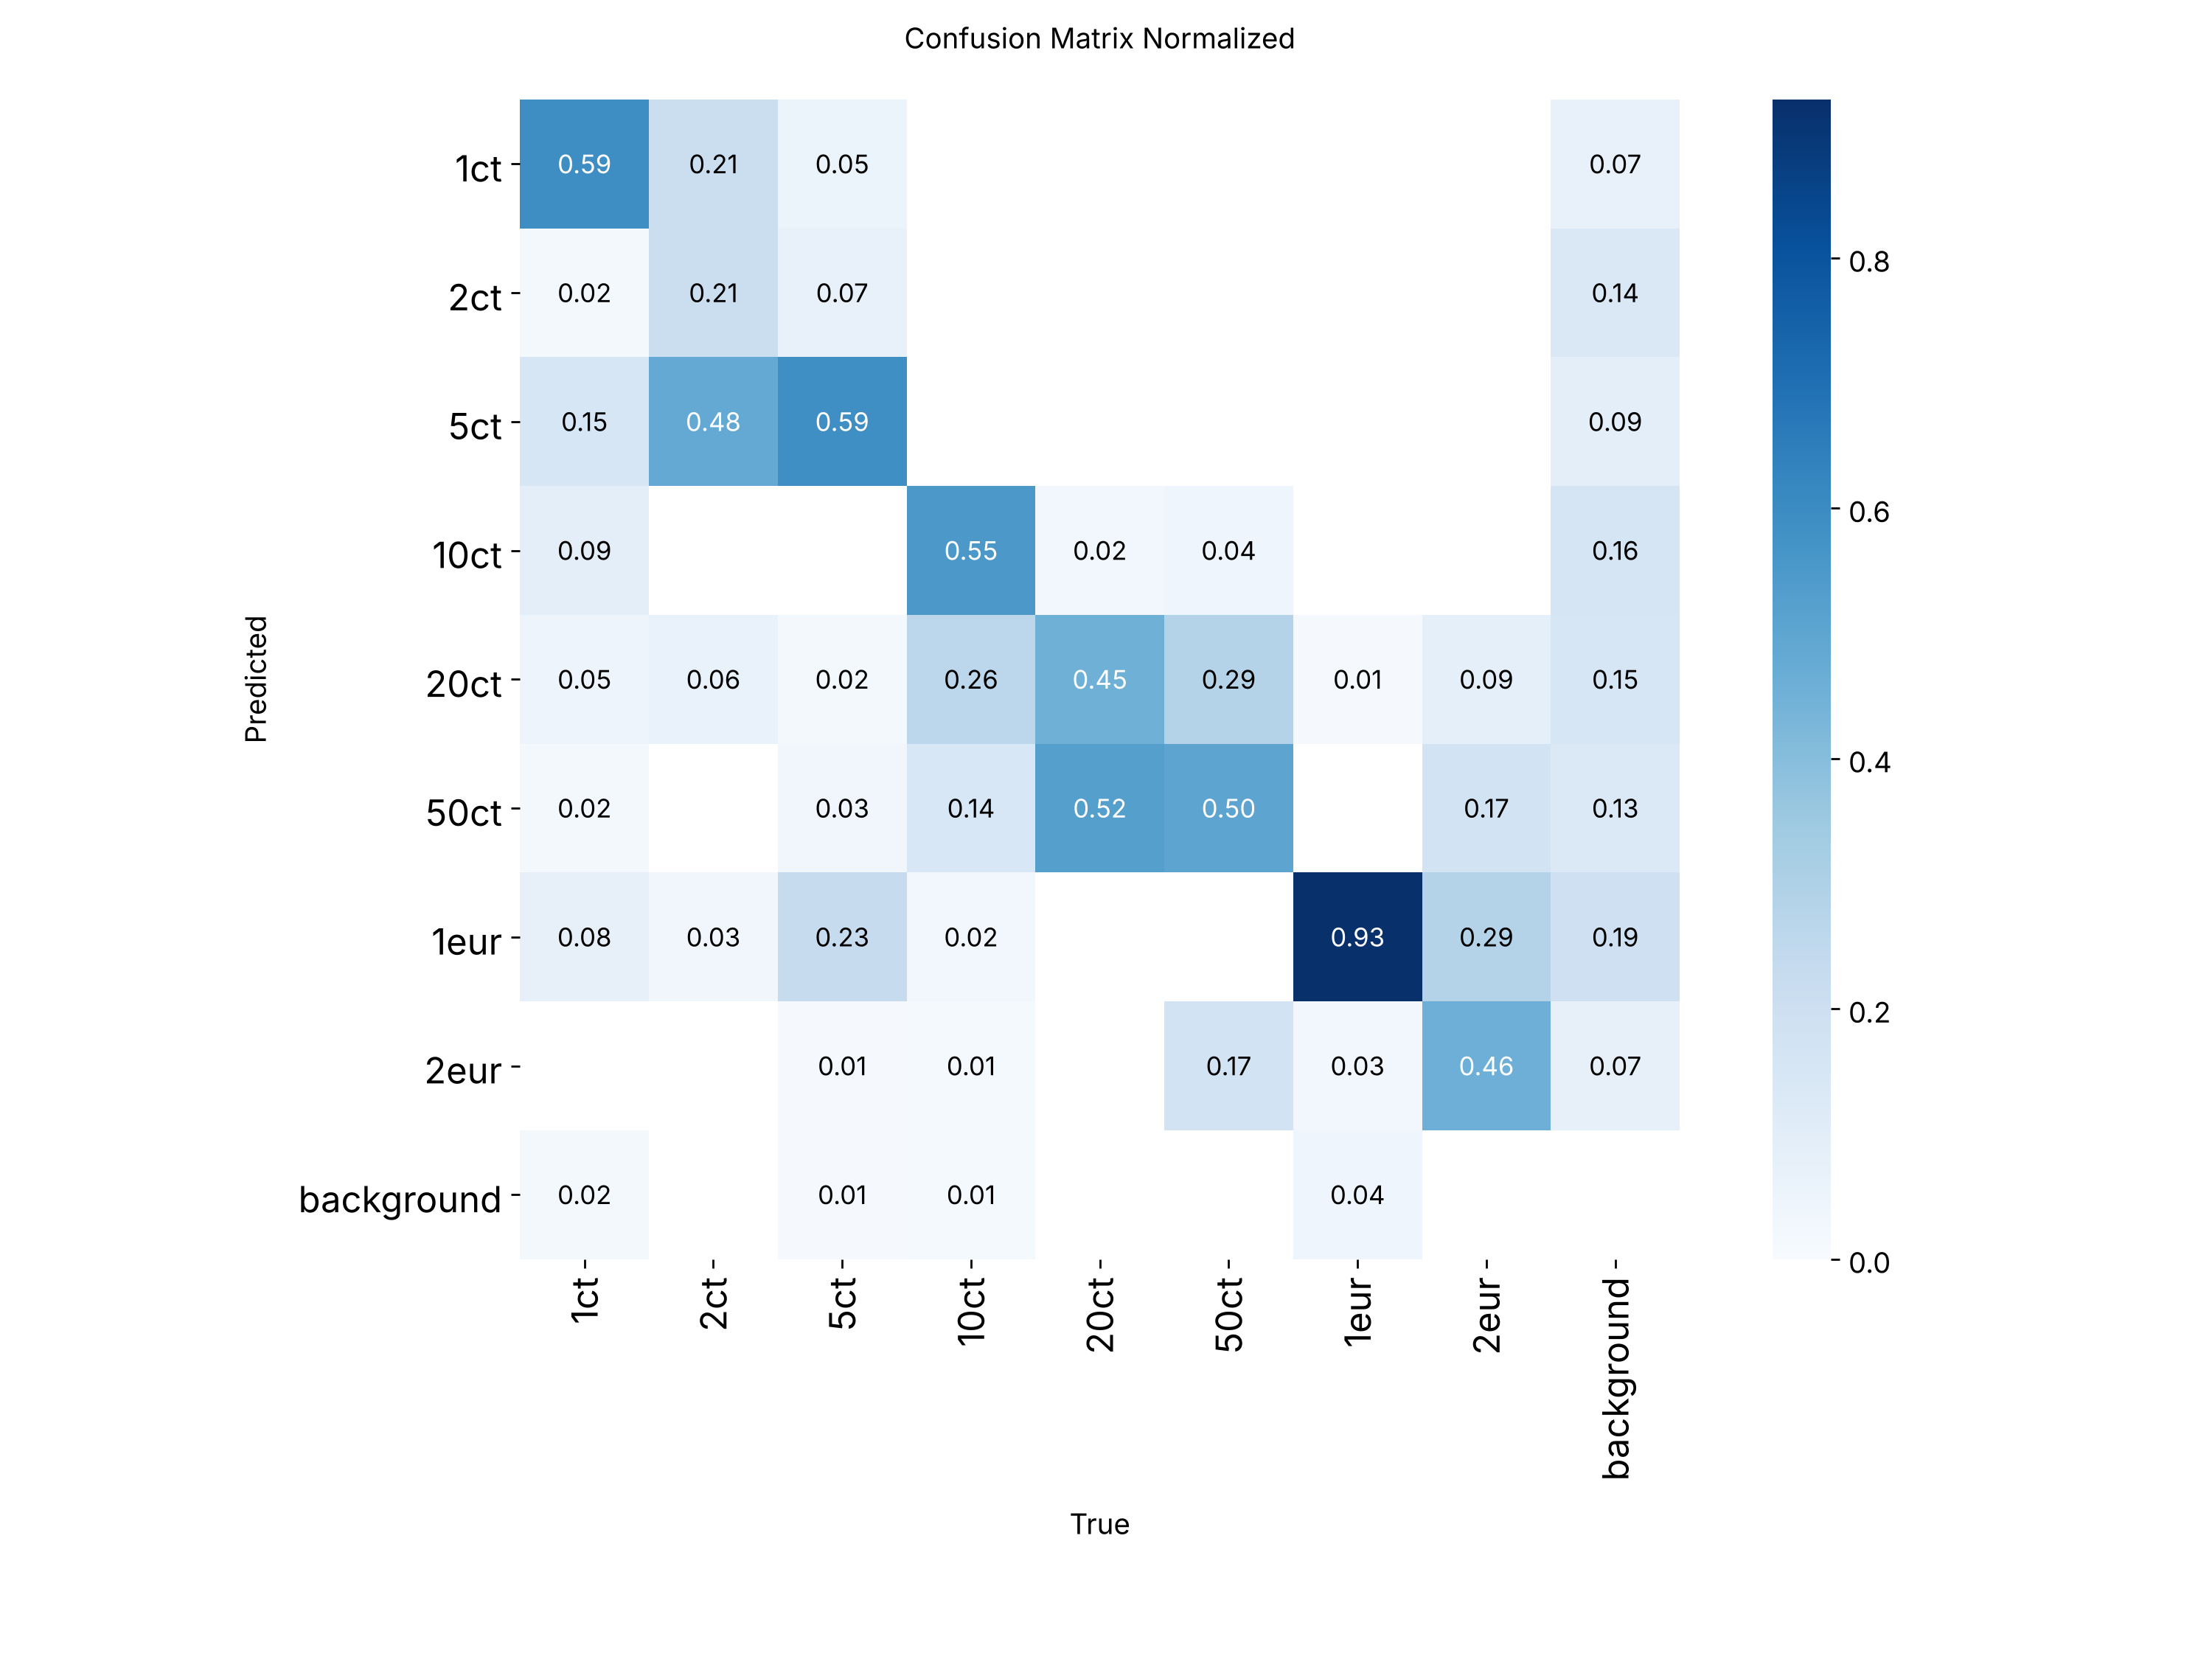
\includegraphics[width=0.9\linewidth]{figures/yolo_confusion.png}

\scriptsize Konfusionsmatrix mit Klasse \texttt{background}
\end{column}
\end{columns}
\source{\cite{ultralytics_val}}
\end{frame}

% ---------------------------------------------------------
\begin{frame}{Anwendungsnahe Metrik: Stimmt der Betrag?}
\footnotesize
\setbeamerfont{block title}{size=\footnotesize}
\begin{columns}
\begin{column}{0.47\textwidth}
\begin{itemize}
  \item Die mAP bewertet die Erkennung, aber nicht den \textbf{Nutzen}.
  \item Für die KI-Kasse zählt: Ist die \textbf{Summe} pro Bild richtig?
  \item Ein einziger Fehlalarm oder eine übersehene Münze macht das Ergebnis falsch.
  \item Der Schwellenwert \texttt{conf} wird so gewählt, dass möglichst viele Beträge stimmen.
  \item Unser Test: mAP@0.5 von 0,49, aber nur bei \textbf{19 von 71} Testbildern mit Münzen stimmt der Betrag exakt.
\end{itemize}
\end{column}
\begin{column}{0.48\textwidth}
\begin{blockC3}{Metrik für die KI-Kasse}
\[
\text{Anteil exakt} = \frac{\#\{\text{Bilder mit korrekter Summe}\}}{\#\{\text{Bilder}\}}
\]
\end{blockC3}
\begin{itemize}
  \item Zusätzlich: mittlerer absoluter Fehler in Euro
  \item Die Bilder mit dem größten Fehler sind der Startpunkt der \textbf{Fehleranalyse}.
\end{itemize}
\end{column}
\end{columns}
\end{frame}

% ---------------------------------------------------------
\begin{frame}{Fehleranalyse und Domain Shift}
\footnotesize
\begin{columns}
\begin{column}{0.47\textwidth}
\begin{itemize}
  \item \textbf{Domain Shift:} Die Einsatzumgebung unterscheidet sich von den Trainingsdaten, z.\,B. Licht im Hörsaal oder eine andere Kamera.
  \item \textbf{Live-Testset:} Bilder der Live-Kamera aufnehmen, etwa 50 annotieren
  \item mAP auf Validierungsdaten und auf dem Live-Testset vergleichen
  \item Die Lücke zeigt, wie gut das Modell \textbf{generalisiert}.
  \item 20 bis 30 Bilder aus der Einsatzumgebung ins Training aufnehmen, neu trainieren, erneut messen
\end{itemize}
\end{column}
\begin{column}{0.48\textwidth}
\centering
\resizebox{0.9\linewidth}{!}{%
\begin{tikzpicture}[schritt/.style={draw, rounded corners=3pt, fill=SecondaryColor!20, font=\small, minimum width=2.4cm, minimum height=0.7cm, align=center}]
  \node[schritt] (a) at (90:2.6) {Live-Bilder\\aufnehmen};
  \node[schritt] (b) at (18:3.2) {Fehler\\analysieren};
  \node[schritt] (c) at (-54:2.9) {Daten\\ergänzen};
  \node[schritt] (d) at (-126:2.9) {neu\\trainieren};
  \node[schritt] (e) at (162:3.2) {erneut\\bewerten};
  \foreach \x/\y in {a/b, b/c, c/d, d/e, e/a}
    \draw[-{Latex[length=2mm]}, line width=0.8pt, PrimaryColor] (\x) -- (\y);
\end{tikzpicture}%
}
\end{column}
\end{columns}
\end{frame}

% ---------------------------------------------------------
\begin{frame}{Aufgabe: Modell bewerten}
\footnotesize
\begin{columns}
\begin{column}{0.60\textwidth}
\begin{enumerate}
  \item Berechnen Sie Precision, Recall und AP für das Beispiel der Klasse 1\,€ in Python und zeichnen Sie die PR-Kurve.
  \item Bewerten Sie Ihr trainiertes Modell mit \texttt{model.val()} auf den Testdaten. Welche Klassen schneiden am schlechtesten ab?
  \item Interpretieren Sie die Konfusionsmatrix. Welche Münzen werden verwechselt?
  \item Bestimmen Sie den Anteil der Testbilder, bei denen die Summe exakt stimmt, und analysieren Sie die Bilder mit dem größten Fehler.
\end{enumerate}
\end{column}
\begin{column}{0.35\textwidth}
\centering
\twemoji[width=0.9\linewidth]{laptop}
\end{column}
\end{columns}
\source{Lösung: \texttt{LösungYoloEvaluation.ipynb}}
\end{frame}

\makesubsectionpage{Deployment und Ausblick}

% ---------------------------------------------------------
\begin{frame}[fragile]{Live-Demo: Die KI-Kasse}
\footnotesize
\begin{columns}
\begin{column}{0.47\textwidth}
{\footnotesize
\begin{minted}{python}
for r in model.predict(source=0,
                       stream=True,
                       conf=conf):
    total = sum(VALUES[r.names[int(c)]]
                for c in r.boxes.cls)
    image = r.plot()
    # Summe einblenden, anzeigen
\end{minted}
}
\begin{itemize}
  \item Skript \texttt{KiKasse.py} mit Reglern für \texttt{conf} und \texttt{iou}
  \item Taste \texttt{n}: NMS ein und aus
  \item Taste \texttt{s}: Bild für das Live-Testset speichern
\end{itemize}

\note{
\begin{itemize}
  \item Das Foto stammt nicht aus dem Datensatz: anderer Untergrund, andere Kamera, andere Beleuchtung.
  \item Die beiden 2-€-Münzen und die 1-€-Münze werden erkannt.
  \item 20 ct und 10 ct werden übersehen, die Kupfermünze wird als 2\,€ erkannt.
  \item Auf der 1-€-Münze liegen zwei Boxen mit verschiedenen Klassen. NMS läuft pro Klasse und entfernt keine davon.
  \item Ergebnis: 9,00\,€ statt rund 5,30\,€, ein typischer Domain Shift.
\end{itemize}
}
\end{column}
\begin{column}{0.48\textwidth}
\centering
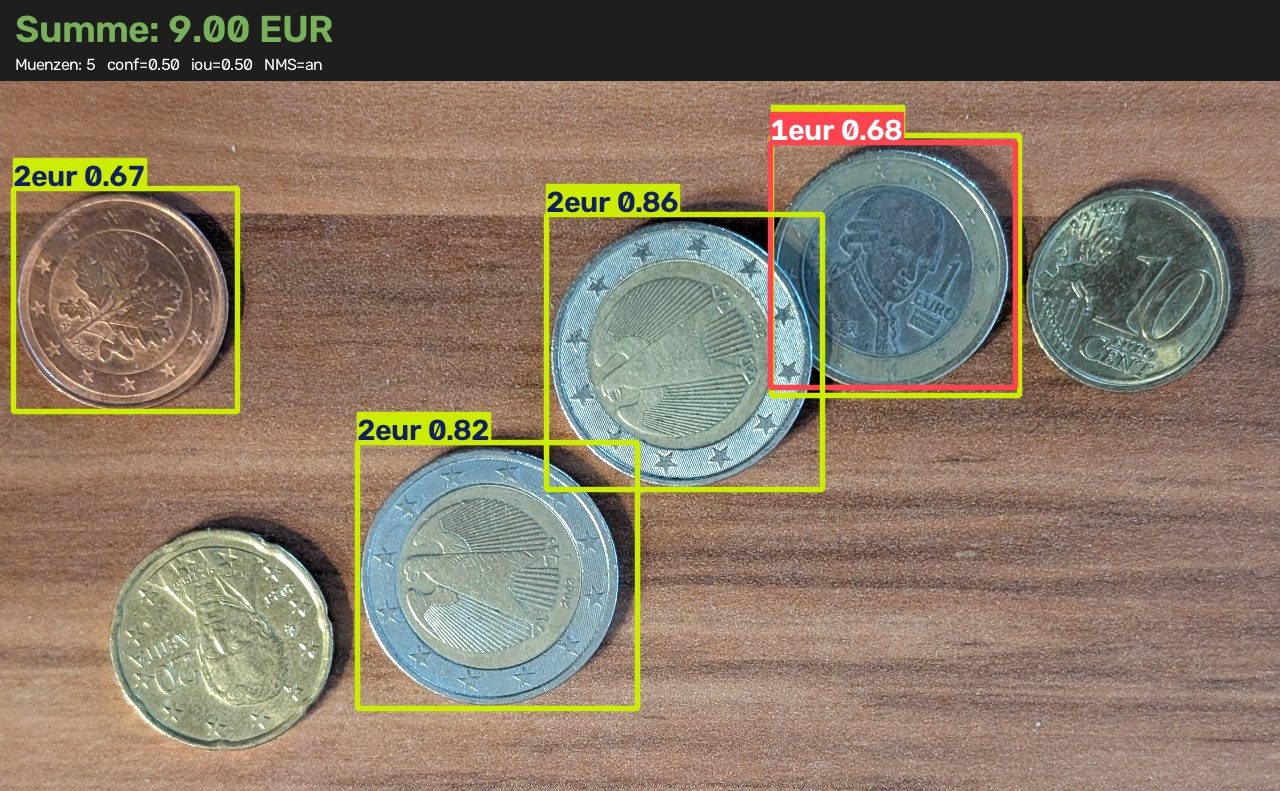
\includegraphics[width=0.9\linewidth]{figures/yolo_kikasse.jpg}

\scriptsize Eigenes Foto, nicht aus dem Datensatz: 9,00\,€ statt rund 5,30\,€
\end{column}
\end{columns}
\end{frame}

% ---------------------------------------------------------
\begin{frame}{Modell exportieren}
\footnotesize
\begin{columns}
\begin{column}{0.47\textwidth}
\begin{itemize}
  \item \texttt{model.export(format="onnx")} erzeugt ein Modell, das ohne PyTorch läuft.
  \item Das exportierte Modell wird wieder mit \texttt{YOLO(...)} geladen.
  \item \texttt{int8=True}: Gewichte mit 8 Bit, kleiner und schneller
  \item \texttt{nms=False}: Bei YOLO26 wird der NMS-freie Head exportiert.
\end{itemize}
\end{column}
\begin{column}{0.48\textwidth}
\centering
\begin{tabular}{ll}
\toprule
\textbf{Ziel} & \textbf{Format} \\
\midrule
Plattformunabhängig & \texttt{onnx} \\
NVIDIA-GPU, Jetson & \texttt{engine} (TensorRT) \\
Intel-CPU & \texttt{openvino} \\
Android, Raspberry Pi & \texttt{tflite} \\
iPhone, Mac & \texttt{coreml} \\
\bottomrule
\end{tabular}

\vspace{0.8em}
Unser Test auf einer CPU: PyTorch 81\,ms, ONNX 68\,ms pro Bild
\end{column}
\end{columns}
\source{\cite{ultralytics_export, ultralytics_yolo26}}
\end{frame}

% ---------------------------------------------------------
\begin{frame}{Weitere Aufgaben mit YOLO}
\footnotesize
\begin{columns}
\begin{column}{0.60\textwidth}
\begin{itemize}
  \item YOLO26 unterstützt sieben Aufgaben mit derselben API:
  \begin{itemize}
    \item Objekterkennung
    \item Instanz- und semantische Segmentierung
    \item Bildklassifikation
    \item Pose-Erkennung, z.\,B. Gelenkpunkte von Menschen
    \item Gedrehte Boxen (OBB), z.\,B. in Luftbildern
    \item Monokulare Tiefenschätzung
  \end{itemize}
  \item \textbf{Open Vocabulary} mit YOLOE-26: Klassen werden per \textbf{Textprompt} vorgegeben, ohne neues Training.
\end{itemize}
\end{column}
\begin{column}{0.35\textwidth}
\centering
\twemoji[width=0.8\linewidth]{rocket}
\end{column}
\end{columns}
\source{\cite{ultralytics_yolo26}}
\end{frame}

% ---------------------------------------------------------
\begin{frame}{Recht und Ethik}
\footnotesize
\setbeamerfont{block title}{size=\footnotesize}
\begin{columns}
\begin{column}{0.60\textwidth}
\begin{itemize}
  \item \textbf{Lizenz:} Ultralytics steht unter AGPL-3.0. Wer ein Produkt damit vertreibt, muss den Quellcode offenlegen oder eine Enterprise-Lizenz erwerben.
  \item \textbf{Datenschutz:} Kamerabilder mit Personen sind personenbezogene Daten im Sinne der DSGVO.
  \item \textbf{EU AI Act:} Bestimmte Anwendungen wie die biometrische Fernidentifizierung in Echtzeit sind stark eingeschränkt.
  \item \textbf{Verzerrungen:} Ein Modell ist nur so ausgewogen wie seine Trainingsdaten.
  \item \textbf{Verantwortung:} Fehlerraten kennen und kommunizieren, gerade wenn Entscheidungen von der Erkennung abhängen
\end{itemize}
\end{column}
\begin{column}{0.35\textwidth}
\centering
\twemoji[width=0.8\linewidth]{balance scale}
\end{column}
\end{columns}
\end{frame}

% ---------------------------------------------------------
\begin{frame}{Zusammenfassung}
\footnotesize
\begin{columns}
\begin{column}{0.47\textwidth}
\begin{itemize}
  \item Objekterkennung: \textbf{Klasse und Box} für jedes Objekt
  \item Grundbegriffe: Box-Formate, \textbf{IoU}, Confidence, \textbf{NMS}
  \item YOLO: ein Durchlauf, drei Skalen, anchor-free, bei YOLO26 optional ohne NMS
  \item Praxis: Daten sind der aufwendigste und wichtigste Teil.
  \item Bewertung mit \textbf{mAP} und einer anwendungsnahen Metrik
  \item Live-Test deckt den \textbf{Domain Shift} auf.
\end{itemize}
\end{column}
\begin{column}{0.48\textwidth}
\centering
\resizebox{0.9\linewidth}{!}{%
\begin{tikzpicture}[schritt/.style={draw, rounded corners=3pt, font=\small, minimum width=3.2cm, minimum height=0.65cm}]
  \node[schritt, fill=SecondaryColor!20] (a) at (0,4) {Daten aufnehmen};
  \node[schritt, fill=SecondaryColor!20] (b) at (0,3) {Annotieren};
  \node[schritt, fill=AccentColor!30] (c) at (0,2) {Trainieren};
  \node[schritt, fill=ExampleColor!35] (d) at (0,1) {Bewerten};
  \node[schritt, fill=ThirdColor!25] (e) at (0,0) {Exportieren und einsetzen};
  \foreach \x/\y in {a/b, b/c, c/d, d/e}
    \draw[-{Latex[length=2mm]}, line width=0.8pt] (\x) -- (\y);
  \draw[-{Latex[length=2mm]}, line width=0.8pt, AlertColor] (e.east) -- ++(0.6,0) |- node[pos=0.25, right, font=\scriptsize, align=left] {Live-Test,\\neue Daten} (a.east);
\end{tikzpicture}%
}
\end{column}
\end{columns}
\end{frame}

% ---------------------------------------------------------
\begin{frame}{Aufgabe: Die KI-Kasse live}
\footnotesize
\begin{columns}
\begin{column}{0.60\textwidth}
\begin{enumerate}
  \item Exportieren Sie Ihr bestes Modell nach ONNX und vergleichen Sie die Laufzeit mit dem PyTorch-Modell.
  \item Starten Sie \texttt{KiKasse.py} mit Ihrer Webcam und testen Sie verschiedene Werte für \texttt{conf} und \texttt{iou}.
  \item Nehmen Sie mit der Taste \texttt{s} mindestens 30 Bilder auf, annotieren Sie diese und bestimmen Sie die mAP auf diesem Live-Testset.
  \item Ergänzen Sie das Training um 20 bis 30 weitere Bilder aus dem Hörsaal und vergleichen Sie die mAP auf dem Live-Testset vor und nach dem Nachtraining.
\end{enumerate}
\end{column}
\begin{column}{0.35\textwidth}
\centering
\twemoji[width=0.9\linewidth]{laptop}
\end{column}
\end{columns}
\source{Lösung: \texttt{LösungYoloExport.ipynb}, \texttt{KiKasse.py}}
\end{frame}
